% !TeX root = Master.tex
\section{Detailed results}
\label{app:complete-results}

This appendix complements Section~\ref{sec:results} with detailed MSE, rank-correlation, and rank-movement results, together with distributions of rank correlations, for all four ACIC error structures and all four N\&W designs at both sample sizes.

\newgeometry{top=10mm,bottom=10mm,left=12mm,right=12mm}
\begin{landscape}
\begingroup
\renewcommand{\papertablestyle}{\fontsize{7.5}{10}\selectfont\setlength{\tabcolsep}{0.5pt}\renewcommand{\arraystretch}{1}}
\begin{longtable}{*{7}{c}@{\hspace{6pt}}*{7}{c}@{\hspace{6pt}}*{7}{c}@{\hspace{6pt}}*{7}{c}}
\caption{Average Monte Carlo MSE by estimator and benchmark, averaged over 100 reference datasets per setting. Each setting has its own estimator order, from lowest to highest target-benchmark MSE.}\label{tab:results_mse_all} \\
\toprule
\makebox[54pt][c]{Estimator} & \makebox[19pt][c]{Target} & \makebox[19pt][c]{GB} & \makebox[19pt][c]{NN} & \makebox[19pt][c]{OLS2} & \makebox[19pt][c]{RF} & \makebox[19pt][c]{WGAN} & \makebox[54pt][c]{Estimator} & \makebox[19pt][c]{Target} & \makebox[19pt][c]{GB} & \makebox[19pt][c]{NN} & \makebox[19pt][c]{OLS2} & \makebox[19pt][c]{RF} & \makebox[19pt][c]{WGAN} & \makebox[54pt][c]{Estimator} & \makebox[19pt][c]{Target} & \makebox[19pt][c]{GB} & \makebox[19pt][c]{NN} & \makebox[19pt][c]{OLS2} & \makebox[19pt][c]{RF} & \makebox[19pt][c]{WGAN} & \makebox[54pt][c]{Estimator} & \makebox[19pt][c]{Target} & \makebox[19pt][c]{GB} & \makebox[19pt][c]{NN} & \makebox[19pt][c]{OLS2} & \makebox[19pt][c]{RF} & \makebox[19pt][c]{WGAN} \\
\midrule
\endfirsthead
\caption[]{Average Monte Carlo MSE by estimator and benchmark, averaged over 100 reference datasets per setting (continued).} \\
\toprule
\makebox[54pt][c]{Estimator} & \makebox[19pt][c]{Target} & \makebox[19pt][c]{GB} & \makebox[19pt][c]{NN} & \makebox[19pt][c]{OLS2} & \makebox[19pt][c]{RF} & \makebox[19pt][c]{WGAN} & \makebox[54pt][c]{Estimator} & \makebox[19pt][c]{Target} & \makebox[19pt][c]{GB} & \makebox[19pt][c]{NN} & \makebox[19pt][c]{OLS2} & \makebox[19pt][c]{RF} & \makebox[19pt][c]{WGAN} & \makebox[54pt][c]{Estimator} & \makebox[19pt][c]{Target} & \makebox[19pt][c]{GB} & \makebox[19pt][c]{NN} & \makebox[19pt][c]{OLS2} & \makebox[19pt][c]{RF} & \makebox[19pt][c]{WGAN} & \makebox[54pt][c]{Estimator} & \makebox[19pt][c]{Target} & \makebox[19pt][c]{GB} & \makebox[19pt][c]{NN} & \makebox[19pt][c]{OLS2} & \makebox[19pt][c]{RF} & \makebox[19pt][c]{WGAN} \\
\midrule
\endhead
\midrule
\multicolumn{28}{r}{Continued on next page} \\
\endfoot
\bottomrule
\endlastfoot
\multicolumn{7}{c}{\textit{ACIC IID}} & \multicolumn{7}{c}{\textit{ACIC Non-additive}} & \multicolumn{7}{c}{\textit{ACIC Group-correlated}} & \multicolumn{7}{c}{\textit{ACIC Heteroskedastic}} \\*
\cmidrule(lr){1-7}\cmidrule(lr){8-14}\cmidrule(lr){15-21}\cmidrule(lr){22-28}
\makebox[54pt][c]{GB G-comp} & \makebox[19pt][c]{0.013} & \makebox[19pt][c]{0.020} & \makebox[19pt][c]{0.041} & \makebox[19pt][c]{0.014} & \makebox[19pt][c]{0.025} & \makebox[19pt][c]{1.879} & \makebox[54pt][c]{GB G-comp} & \makebox[19pt][c]{0.021} & \makebox[19pt][c]{0.035} & \makebox[19pt][c]{0.064} & \makebox[19pt][c]{0.026} & \makebox[19pt][c]{0.065} & \makebox[19pt][c]{3.521} & \makebox[54pt][c]{GB G-comp} & \makebox[19pt][c]{0.011} & \makebox[19pt][c]{0.017} & \makebox[19pt][c]{0.041} & \makebox[19pt][c]{0.012} & \makebox[19pt][c]{0.021} & \makebox[19pt][c]{1.804} & \makebox[54pt][c]{GB G-comp} & \makebox[19pt][c]{0.012} & \makebox[19pt][c]{0.020} & \makebox[19pt][c]{0.042} & \makebox[19pt][c]{0.014} & \makebox[19pt][c]{0.023} & \makebox[19pt][c]{1.771} \\*
\makebox[54pt][c]{BCF G-comp} & \makebox[19pt][c]{0.015} & \makebox[19pt][c]{0.019} & \makebox[19pt][c]{0.034} & \makebox[19pt][c]{0.018} & \makebox[19pt][c]{0.040} & \makebox[19pt][c]{2.222} & \makebox[54pt][c]{BCF G-comp} & \makebox[19pt][c]{0.029} & \makebox[19pt][c]{0.033} & \makebox[19pt][c]{0.054} & \makebox[19pt][c]{0.034} & \makebox[19pt][c]{0.105} & \makebox[19pt][c]{4.100} & \makebox[54pt][c]{BCF G-comp} & \makebox[19pt][c]{0.014} & \makebox[19pt][c]{0.016} & \makebox[19pt][c]{0.029} & \makebox[19pt][c]{0.016} & \makebox[19pt][c]{0.041} & \makebox[19pt][c]{2.106} & \makebox[54pt][c]{BCF G-comp} & \makebox[19pt][c]{0.015} & \makebox[19pt][c]{0.018} & \makebox[19pt][c]{0.033} & \makebox[19pt][c]{0.018} & \makebox[19pt][c]{0.039} & \makebox[19pt][c]{2.132} \\*
\makebox[54pt][c]{GB--OLS2 AIPW} & \makebox[19pt][c]{0.022} & \makebox[19pt][c]{0.030} & \makebox[19pt][c]{0.043} & \makebox[19pt][c]{0.030} & \makebox[19pt][c]{0.035} & \makebox[19pt][c]{1.623} & \makebox[54pt][c]{GB--OLS2 AIPW} & \makebox[19pt][c]{0.036} & \makebox[19pt][c]{0.051} & \makebox[19pt][c]{0.070} & \makebox[19pt][c]{0.054} & \makebox[19pt][c]{0.079} & \makebox[19pt][c]{3.096} & \makebox[54pt][c]{GB--OLS2 AIPW} & \makebox[19pt][c]{0.019} & \makebox[19pt][c]{0.025} & \makebox[19pt][c]{0.042} & \makebox[19pt][c]{0.027} & \makebox[19pt][c]{0.030} & \makebox[19pt][c]{1.638} & \makebox[54pt][c]{GB--OLS2 AIPW} & \makebox[19pt][c]{0.021} & \makebox[19pt][c]{0.028} & \makebox[19pt][c]{0.043} & \makebox[19pt][c]{0.029} & \makebox[19pt][c]{0.033} & \makebox[19pt][c]{1.611} \\*
\makebox[54pt][c]{GB--GB AIPW} & \makebox[19pt][c]{0.027} & \makebox[19pt][c]{0.031} & \makebox[19pt][c]{0.033} & \makebox[19pt][c]{0.037} & \makebox[19pt][c]{0.055} & \makebox[19pt][c]{1.161} & \makebox[54pt][c]{GB--GB AIPW} & \makebox[19pt][c]{0.044} & \makebox[19pt][c]{0.052} & \makebox[19pt][c]{0.056} & \makebox[19pt][c]{0.067} & \makebox[19pt][c]{0.121} & \makebox[19pt][c]{2.200} & \makebox[54pt][c]{NN G-comp} & \makebox[19pt][c]{0.022} & \makebox[19pt][c]{0.054} & \makebox[19pt][c]{0.078} & \makebox[19pt][c]{0.010} & \makebox[19pt][c]{0.046} & \makebox[19pt][c]{1.400} & \makebox[54pt][c]{GB--GB AIPW} & \makebox[19pt][c]{0.025} & \makebox[19pt][c]{0.029} & \makebox[19pt][c]{0.031} & \makebox[19pt][c]{0.036} & \makebox[19pt][c]{0.052} & \makebox[19pt][c]{1.135} \\*
\makebox[54pt][c]{GB--RF AIPW} & \makebox[19pt][c]{0.027} & \makebox[19pt][c]{0.034} & \makebox[19pt][c]{0.043} & \makebox[19pt][c]{0.047} & \makebox[19pt][c]{0.044} & \makebox[19pt][c]{1.240} & \makebox[54pt][c]{GB--RF AIPW} & \makebox[19pt][c]{0.045} & \makebox[19pt][c]{0.059} & \makebox[19pt][c]{0.071} & \makebox[19pt][c]{0.086} & \makebox[19pt][c]{0.084} & \makebox[19pt][c]{2.218} & \makebox[54pt][c]{GB--GB AIPW} & \makebox[19pt][c]{0.022} & \makebox[19pt][c]{0.026} & \makebox[19pt][c]{0.029} & \makebox[19pt][c]{0.033} & \makebox[19pt][c]{0.049} & \makebox[19pt][c]{1.099} & \makebox[54pt][c]{GB--RF AIPW} & \makebox[19pt][c]{0.026} & \makebox[19pt][c]{0.033} & \makebox[19pt][c]{0.042} & \makebox[19pt][c]{0.047} & \makebox[19pt][c]{0.042} & \makebox[19pt][c]{1.199} \\*
\makebox[54pt][c]{NN G-comp} & \makebox[19pt][c]{0.039} & \makebox[19pt][c]{0.095} & \makebox[19pt][c]{0.112} & \makebox[19pt][c]{0.012} & \makebox[19pt][c]{0.081} & \makebox[19pt][c]{1.474} & \makebox[54pt][c]{GB--NN AIPW} & \makebox[19pt][c]{0.069} & \makebox[19pt][c]{0.065} & \makebox[19pt][c]{0.048} & \makebox[19pt][c]{0.056} & \makebox[19pt][c]{0.153} & \makebox[19pt][c]{1.834} & \makebox[54pt][c]{GB--RF AIPW} & \makebox[19pt][c]{0.022} & \makebox[19pt][c]{0.029} & \makebox[19pt][c]{0.039} & \makebox[19pt][c]{0.043} & \makebox[19pt][c]{0.038} & \makebox[19pt][c]{1.188} & \makebox[54pt][c]{NN G-comp} & \makebox[19pt][c]{0.032} & \makebox[19pt][c]{0.081} & \makebox[19pt][c]{0.102} & \makebox[19pt][c]{0.011} & \makebox[19pt][c]{0.070} & \makebox[19pt][c]{1.382} \\*
\makebox[54pt][c]{GB--NN AIPW} & \makebox[19pt][c]{0.042} & \makebox[19pt][c]{0.040} & \makebox[19pt][c]{0.027} & \makebox[19pt][c]{0.031} & \makebox[19pt][c]{0.071} & \makebox[19pt][c]{0.926} & \makebox[54pt][c]{NN G-comp} & \makebox[19pt][c]{0.069} & \makebox[19pt][c]{0.175} & \makebox[19pt][c]{0.200} & \makebox[19pt][c]{0.023} & \makebox[19pt][c]{0.119} & \makebox[19pt][c]{2.905} & \makebox[54pt][c]{GB--NN AIPW} & \makebox[19pt][c]{0.040} & \makebox[19pt][c]{0.038} & \makebox[19pt][c]{0.022} & \makebox[19pt][c]{0.028} & \makebox[19pt][c]{0.072} & \makebox[19pt][c]{0.874} & \makebox[54pt][c]{GB--NN AIPW} & \makebox[19pt][c]{0.042} & \makebox[19pt][c]{0.038} & \makebox[19pt][c]{0.025} & \makebox[19pt][c]{0.031} & \makebox[19pt][c]{0.071} & \makebox[19pt][c]{0.898} \\*
\makebox[54pt][c]{RF G-comp} & \makebox[19pt][c]{0.063} & \makebox[19pt][c]{0.076} & \makebox[19pt][c]{0.105} & \makebox[19pt][c]{0.021} & \makebox[19pt][c]{0.024} & \makebox[19pt][c]{2.367} & \makebox[54pt][c]{GB--GB TMLE} & \makebox[19pt][c]{0.109} & \makebox[19pt][c]{0.132} & \makebox[19pt][c]{0.102} & \makebox[19pt][c]{0.149} & \makebox[19pt][c]{0.222} & \makebox[19pt][c]{1.292} & \makebox[54pt][c]{GB--GB TMLE} & \makebox[19pt][c]{0.057} & \makebox[19pt][c]{0.069} & \makebox[19pt][c]{0.046} & \makebox[19pt][c]{0.074} & \makebox[19pt][c]{0.101} & \makebox[19pt][c]{0.633} & \makebox[54pt][c]{RF G-comp} & \makebox[19pt][c]{0.059} & \makebox[19pt][c]{0.073} & \makebox[19pt][c]{0.107} & \makebox[19pt][c]{0.021} & \makebox[19pt][c]{0.023} & \makebox[19pt][c]{2.245} \\*
\makebox[54pt][c]{GB--GB TMLE} & \makebox[19pt][c]{0.067} & \makebox[19pt][c]{0.080} & \makebox[19pt][c]{0.056} & \makebox[19pt][c]{0.083} & \makebox[19pt][c]{0.113} & \makebox[19pt][c]{0.699} & \makebox[54pt][c]{RF G-comp} & \makebox[19pt][c]{0.155} & \makebox[19pt][c]{0.146} & \makebox[19pt][c]{0.166} & \makebox[19pt][c]{0.039} & \makebox[19pt][c]{0.033} & \makebox[19pt][c]{4.147} & \makebox[54pt][c]{RF G-comp} & \makebox[19pt][c]{0.060} & \makebox[19pt][c]{0.071} & \makebox[19pt][c]{0.109} & \makebox[19pt][c]{0.019} & \makebox[19pt][c]{0.021} & \makebox[19pt][c]{2.373} & \makebox[54pt][c]{GB--GB TMLE} & \makebox[19pt][c]{0.063} & \makebox[19pt][c]{0.074} & \makebox[19pt][c]{0.052} & \makebox[19pt][c]{0.081} & \makebox[19pt][c]{0.107} & \makebox[19pt][c]{0.688} \\*
\makebox[54pt][c]{GB--RF TMLE} & \makebox[19pt][c]{0.097} & \makebox[19pt][c]{0.107} & \makebox[19pt][c]{0.070} & \makebox[19pt][c]{0.102} & \makebox[19pt][c]{0.148} & \makebox[19pt][c]{0.605} & \makebox[54pt][c]{GB--RF TMLE} & \makebox[19pt][c]{0.157} & \makebox[19pt][c]{0.176} & \makebox[19pt][c]{0.128} & \makebox[19pt][c]{0.183} & \makebox[19pt][c]{0.284} & \makebox[19pt][c]{1.069} & \makebox[54pt][c]{GB--RF TMLE} & \makebox[19pt][c]{0.086} & \makebox[19pt][c]{0.095} & \makebox[19pt][c]{0.059} & \makebox[19pt][c]{0.092} & \makebox[19pt][c]{0.132} & \makebox[19pt][c]{0.526} & \makebox[54pt][c]{GB--RF TMLE} & \makebox[19pt][c]{0.092} & \makebox[19pt][c]{0.100} & \makebox[19pt][c]{0.065} & \makebox[19pt][c]{0.101} & \makebox[19pt][c]{0.140} & \makebox[19pt][c]{0.583} \\*
\makebox[54pt][c]{GB IPW} & \makebox[19pt][c]{0.106} & \makebox[19pt][c]{0.117} & \makebox[19pt][c]{0.185} & \makebox[19pt][c]{0.122} & \makebox[19pt][c]{0.059} & \makebox[19pt][c]{2.274} & \makebox[54pt][c]{GB IPW} & \makebox[19pt][c]{0.184} & \makebox[19pt][c]{0.211} & \makebox[19pt][c]{0.320} & \makebox[19pt][c]{0.225} & \makebox[19pt][c]{0.078} & \makebox[19pt][c]{4.165} & \makebox[54pt][c]{GB IPW} & \makebox[19pt][c]{0.103} & \makebox[19pt][c]{0.111} & \makebox[19pt][c]{0.184} & \makebox[19pt][c]{0.119} & \makebox[19pt][c]{0.055} & \makebox[19pt][c]{2.219} & \makebox[54pt][c]{GB IPW} & \makebox[19pt][c]{0.105} & \makebox[19pt][c]{0.117} & \makebox[19pt][c]{0.185} & \makebox[19pt][c]{0.121} & \makebox[19pt][c]{0.059} & \makebox[19pt][c]{2.187} \\*
\makebox[54pt][c]{GB--NN TMLE} & \makebox[19pt][c]{0.193} & \makebox[19pt][c]{0.240} & \makebox[19pt][c]{0.121} & \makebox[19pt][c]{0.081} & \makebox[19pt][c]{0.398} & \makebox[19pt][c]{0.574} & \makebox[54pt][c]{GB--NN TMLE} & \makebox[19pt][c]{0.316} & \makebox[19pt][c]{0.403} & \makebox[19pt][c]{0.228} & \makebox[19pt][c]{0.146} & \makebox[19pt][c]{0.779} & \makebox[19pt][c]{1.103} & \makebox[54pt][c]{GB--NN TMLE} & \makebox[19pt][c]{0.152} & \makebox[19pt][c]{0.194} & \makebox[19pt][c]{0.096} & \makebox[19pt][c]{0.072} & \makebox[19pt][c]{0.325} & \makebox[19pt][c]{0.519} & \makebox[54pt][c]{GB--NN TMLE} & \makebox[19pt][c]{0.180} & \makebox[19pt][c]{0.220} & \makebox[19pt][c]{0.113} & \makebox[19pt][c]{0.080} & \makebox[19pt][c]{0.373} & \makebox[19pt][c]{0.558} \\*
\makebox[54pt][c]{GB--OLS2 TMLE} & \makebox[19pt][c]{0.712} & \makebox[19pt][c]{0.662} & \makebox[19pt][c]{0.365} & \makebox[19pt][c]{0.079} & \makebox[19pt][c]{0.812} & \makebox[19pt][c]{0.403} & \makebox[54pt][c]{GB--OLS2 TMLE} & \makebox[19pt][c]{1.252} & \makebox[19pt][c]{1.162} & \makebox[19pt][c]{0.652} & \makebox[19pt][c]{0.143} & \makebox[19pt][c]{1.543} & \makebox[19pt][c]{0.824} & \makebox[54pt][c]{GB--OLS2 TMLE} & \makebox[19pt][c]{0.701} & \makebox[19pt][c]{0.658} & \makebox[19pt][c]{0.390} & \makebox[19pt][c]{0.071} & \makebox[19pt][c]{0.802} & \makebox[19pt][c]{0.347} & \makebox[54pt][c]{GB--OLS2 TMLE} & \makebox[19pt][c]{0.709} & \makebox[19pt][c]{0.654} & \makebox[19pt][c]{0.373} & \makebox[19pt][c]{0.078} & \makebox[19pt][c]{0.808} & \makebox[19pt][c]{0.409} \\*
\makebox[54pt][c]{OLS2 G-comp} & \makebox[19pt][c]{0.869} & \makebox[19pt][c]{0.859} & \makebox[19pt][c]{0.777} & \makebox[19pt][c]{0.009} & \makebox[19pt][c]{0.590} & \makebox[19pt][c]{4.795} & \makebox[54pt][c]{OLS2 G-comp} & \makebox[19pt][c]{1.487} & \makebox[19pt][c]{1.498} & \makebox[19pt][c]{1.275} & \makebox[19pt][c]{0.017} & \makebox[19pt][c]{0.866} & \makebox[19pt][c]{8.432} & \makebox[54pt][c]{OLS2 G-comp} & \makebox[19pt][c]{0.867} & \makebox[19pt][c]{0.847} & \makebox[19pt][c]{0.842} & \makebox[19pt][c]{0.008} & \makebox[19pt][c]{0.590} & \makebox[19pt][c]{5.021} & \makebox[54pt][c]{OLS2 G-comp} & \makebox[19pt][c]{0.868} & \makebox[19pt][c]{0.864} & \makebox[19pt][c]{0.813} & \makebox[19pt][c]{0.009} & \makebox[19pt][c]{0.598} & \makebox[19pt][c]{4.614} \\*
\makebox[54pt][c]{OLS1} & \makebox[19pt][c]{0.887} & \makebox[19pt][c]{0.877} & \makebox[19pt][c]{0.795} & \makebox[19pt][c]{0.009} & \makebox[19pt][c]{0.604} & \makebox[19pt][c]{4.842} & \makebox[54pt][c]{OLS1} & \makebox[19pt][c]{1.541} & \makebox[19pt][c]{1.553} & \makebox[19pt][c]{1.327} & \makebox[19pt][c]{0.018} & \makebox[19pt][c]{0.906} & \makebox[19pt][c]{8.648} & \makebox[54pt][c]{OLS1} & \makebox[19pt][c]{0.885} & \makebox[19pt][c]{0.865} & \makebox[19pt][c]{0.861} & \makebox[19pt][c]{0.008} & \makebox[19pt][c]{0.604} & \makebox[19pt][c]{5.075} & \makebox[54pt][c]{OLS1} & \makebox[19pt][c]{0.887} & \makebox[19pt][c]{0.882} & \makebox[19pt][c]{0.831} & \makebox[19pt][c]{0.009} & \makebox[19pt][c]{0.611} & \makebox[19pt][c]{4.683} \\
\addlinespace[14pt]
\multicolumn{7}{c}{\textit{N\&W A, $n=1000$}} & \multicolumn{7}{c}{\textit{N\&W A, $n=4302$}} & \multicolumn{7}{c}{\textit{N\&W B, $n=1000$}} & \multicolumn{7}{c}{\textit{N\&W B, $n=4302$}} \\*
\cmidrule(lr){1-7}\cmidrule(lr){8-14}\cmidrule(lr){15-21}\cmidrule(lr){22-28}
\makebox[54pt][c]{GB G-comp} & \makebox[19pt][c]{0.010} & \makebox[19pt][c]{0.009} & \makebox[19pt][c]{0.008} & \makebox[19pt][c]{0.007} & \makebox[19pt][c]{0.011} & \makebox[19pt][c]{0.003} & \makebox[54pt][c]{GB--GB TMLE} & \makebox[19pt][c]{0.002} & \makebox[19pt][c]{0.003} & \makebox[19pt][c]{0.002} & \makebox[19pt][c]{0.002} & \makebox[19pt][c]{0.005} & \makebox[19pt][c]{0.001} & \makebox[54pt][c]{OLS2 G-comp} & \makebox[19pt][c]{0.004} & \makebox[19pt][c]{0.009} & \makebox[19pt][c]{0.005} & \makebox[19pt][c]{0.005} & \makebox[19pt][c]{0.026} & \makebox[19pt][c]{0.001} & \makebox[54pt][c]{OLS2 G-comp} & \makebox[19pt][c]{0.001} & \makebox[19pt][c]{0.002} & \makebox[19pt][c]{0.001} & \makebox[19pt][c]{0.001} & \makebox[19pt][c]{0.006} & \makebox[19pt][c]{0.000} \\*
\makebox[54pt][c]{GB--GB TMLE} & \makebox[19pt][c]{0.011} & \makebox[19pt][c]{0.015} & \makebox[19pt][c]{0.012} & \makebox[19pt][c]{0.011} & \makebox[19pt][c]{0.017} & \makebox[19pt][c]{0.002} & \makebox[54pt][c]{GB--GB AIPW} & \makebox[19pt][c]{0.002} & \makebox[19pt][c]{0.003} & \makebox[19pt][c]{0.002} & \makebox[19pt][c]{0.002} & \makebox[19pt][c]{0.005} & \makebox[19pt][c]{0.001} & \makebox[54pt][c]{NN G-comp} & \makebox[19pt][c]{0.005} & \makebox[19pt][c]{0.010} & \makebox[19pt][c]{0.005} & \makebox[19pt][c]{0.005} & \makebox[19pt][c]{0.026} & \makebox[19pt][c]{0.001} & \makebox[54pt][c]{GB--NN TMLE} & \makebox[19pt][c]{0.001} & \makebox[19pt][c]{0.002} & \makebox[19pt][c]{0.001} & \makebox[19pt][c]{0.001} & \makebox[19pt][c]{0.006} & \makebox[19pt][c]{0.000} \\*
\makebox[54pt][c]{GB--OLS2 TMLE} & \makebox[19pt][c]{0.011} & \makebox[19pt][c]{0.013} & \makebox[19pt][c]{0.010} & \makebox[19pt][c]{0.010} & \makebox[19pt][c]{0.013} & \makebox[19pt][c]{0.002} & \makebox[54pt][c]{GB IPW} & \makebox[19pt][c]{0.002} & \makebox[19pt][c]{0.002} & \makebox[19pt][c]{0.002} & \makebox[19pt][c]{0.002} & \makebox[19pt][c]{0.004} & \makebox[19pt][c]{0.002} & \makebox[54pt][c]{GB--OLS2 TMLE} & \makebox[19pt][c]{0.005} & \makebox[19pt][c]{0.011} & \makebox[19pt][c]{0.006} & \makebox[19pt][c]{0.006} & \makebox[19pt][c]{0.028} & \makebox[19pt][c]{0.001} & \makebox[54pt][c]{GB--NN AIPW} & \makebox[19pt][c]{0.001} & \makebox[19pt][c]{0.002} & \makebox[19pt][c]{0.001} & \makebox[19pt][c]{0.001} & \makebox[19pt][c]{0.006} & \makebox[19pt][c]{0.000} \\*
\makebox[54pt][c]{GB--NN TMLE} & \makebox[19pt][c]{0.012} & \makebox[19pt][c]{0.012} & \makebox[19pt][c]{0.009} & \makebox[19pt][c]{0.010} & \makebox[19pt][c]{0.013} & \makebox[19pt][c]{0.002} & \makebox[54pt][c]{GB--RF AIPW} & \makebox[19pt][c]{0.002} & \makebox[19pt][c]{0.002} & \makebox[19pt][c]{0.002} & \makebox[19pt][c]{0.002} & \makebox[19pt][c]{0.004} & \makebox[19pt][c]{0.001} & \makebox[54pt][c]{GB--NN TMLE} & \makebox[19pt][c]{0.005} & \makebox[19pt][c]{0.011} & \makebox[19pt][c]{0.006} & \makebox[19pt][c]{0.006} & \makebox[19pt][c]{0.028} & \makebox[19pt][c]{0.001} & \makebox[54pt][c]{GB--OLS2 TMLE} & \makebox[19pt][c]{0.001} & \makebox[19pt][c]{0.002} & \makebox[19pt][c]{0.001} & \makebox[19pt][c]{0.001} & \makebox[19pt][c]{0.006} & \makebox[19pt][c]{0.000} \\*
\makebox[54pt][c]{GB--RF TMLE} & \makebox[19pt][c]{0.012} & \makebox[19pt][c]{0.014} & \makebox[19pt][c]{0.010} & \makebox[19pt][c]{0.011} & \makebox[19pt][c]{0.014} & \makebox[19pt][c]{0.002} & \makebox[54pt][c]{GB--NN AIPW} & \makebox[19pt][c]{0.002} & \makebox[19pt][c]{0.002} & \makebox[19pt][c]{0.002} & \makebox[19pt][c]{0.002} & \makebox[19pt][c]{0.004} & \makebox[19pt][c]{0.001} & \makebox[54pt][c]{OLS1} & \makebox[19pt][c]{0.006} & \makebox[19pt][c]{0.010} & \makebox[19pt][c]{0.006} & \makebox[19pt][c]{0.006} & \makebox[19pt][c]{0.026} & \makebox[19pt][c]{0.001} & \makebox[54pt][c]{GB--OLS2 AIPW} & \makebox[19pt][c]{0.001} & \makebox[19pt][c]{0.002} & \makebox[19pt][c]{0.001} & \makebox[19pt][c]{0.001} & \makebox[19pt][c]{0.006} & \makebox[19pt][c]{0.000} \\*
\makebox[54pt][c]{GB IPW} & \makebox[19pt][c]{0.013} & \makebox[19pt][c]{0.023} & \makebox[19pt][c]{0.017} & \makebox[19pt][c]{0.018} & \makebox[19pt][c]{0.028} & \makebox[19pt][c]{0.007} & \makebox[54pt][c]{BCF G-comp} & \makebox[19pt][c]{0.002} & \makebox[19pt][c]{0.004} & \makebox[19pt][c]{0.002} & \makebox[19pt][c]{0.002} & \makebox[19pt][c]{0.008} & \makebox[19pt][c]{0.002} & \makebox[54pt][c]{GB--OLS2 AIPW} & \makebox[19pt][c]{0.006} & \makebox[19pt][c]{0.013} & \makebox[19pt][c]{0.006} & \makebox[19pt][c]{0.006} & \makebox[19pt][c]{0.030} & \makebox[19pt][c]{0.002} & \makebox[54pt][c]{GB--RF TMLE} & \makebox[19pt][c]{0.001} & \makebox[19pt][c]{0.002} & \makebox[19pt][c]{0.001} & \makebox[19pt][c]{0.001} & \makebox[19pt][c]{0.005} & \makebox[19pt][c]{0.000} \\*
\makebox[54pt][c]{GB--OLS2 AIPW} & \makebox[19pt][c]{0.014} & \makebox[19pt][c]{0.022} & \makebox[19pt][c]{0.015} & \makebox[19pt][c]{0.015} & \makebox[19pt][c]{0.022} & \makebox[19pt][c]{0.004} & \makebox[54pt][c]{GB--OLS2 AIPW} & \makebox[19pt][c]{0.002} & \makebox[19pt][c]{0.002} & \makebox[19pt][c]{0.002} & \makebox[19pt][c]{0.002} & \makebox[19pt][c]{0.003} & \makebox[19pt][c]{0.001} & \makebox[54pt][c]{GB--NN AIPW} & \makebox[19pt][c]{0.006} & \makebox[19pt][c]{0.013} & \makebox[19pt][c]{0.006} & \makebox[19pt][c]{0.007} & \makebox[19pt][c]{0.030} & \makebox[19pt][c]{0.002} & \makebox[54pt][c]{GB--RF AIPW} & \makebox[19pt][c]{0.001} & \makebox[19pt][c]{0.002} & \makebox[19pt][c]{0.001} & \makebox[19pt][c]{0.001} & \makebox[19pt][c]{0.006} & \makebox[19pt][c]{0.000} \\*
\makebox[54pt][c]{OLS2 G-comp} & \makebox[19pt][c]{0.014} & \makebox[19pt][c]{0.010} & \makebox[19pt][c]{0.007} & \makebox[19pt][c]{0.007} & \makebox[19pt][c]{0.008} & \makebox[19pt][c]{0.002} & \makebox[54pt][c]{GB--RF TMLE} & \makebox[19pt][c]{0.002} & \makebox[19pt][c]{0.002} & \makebox[19pt][c]{0.002} & \makebox[19pt][c]{0.002} & \makebox[19pt][c]{0.003} & \makebox[19pt][c]{0.001} & \makebox[54pt][c]{GB--GB TMLE} & \makebox[19pt][c]{0.006} & \makebox[19pt][c]{0.011} & \makebox[19pt][c]{0.007} & \makebox[19pt][c]{0.007} & \makebox[19pt][c]{0.026} & \makebox[19pt][c]{0.002} & \makebox[54pt][c]{GB--GB TMLE} & \makebox[19pt][c]{0.001} & \makebox[19pt][c]{0.002} & \makebox[19pt][c]{0.001} & \makebox[19pt][c]{0.001} & \makebox[19pt][c]{0.006} & \makebox[19pt][c]{0.000} \\*
\makebox[54pt][c]{GB--RF AIPW} & \makebox[19pt][c]{0.014} & \makebox[19pt][c]{0.023} & \makebox[19pt][c]{0.016} & \makebox[19pt][c]{0.017} & \makebox[19pt][c]{0.025} & \makebox[19pt][c]{0.005} & \makebox[54pt][c]{GB--NN TMLE} & \makebox[19pt][c]{0.003} & \makebox[19pt][c]{0.002} & \makebox[19pt][c]{0.002} & \makebox[19pt][c]{0.002} & \makebox[19pt][c]{0.003} & \makebox[19pt][c]{0.001} & \makebox[54pt][c]{GB--RF TMLE} & \makebox[19pt][c]{0.007} & \makebox[19pt][c]{0.009} & \makebox[19pt][c]{0.007} & \makebox[19pt][c]{0.007} & \makebox[19pt][c]{0.020} & \makebox[19pt][c]{0.002} & \makebox[54pt][c]{NN G-comp} & \makebox[19pt][c]{0.001} & \makebox[19pt][c]{0.002} & \makebox[19pt][c]{0.001} & \makebox[19pt][c]{0.001} & \makebox[19pt][c]{0.006} & \makebox[19pt][c]{0.000} \\*
\makebox[54pt][c]{GB--NN AIPW} & \makebox[19pt][c]{0.015} & \makebox[19pt][c]{0.025} & \makebox[19pt][c]{0.016} & \makebox[19pt][c]{0.018} & \makebox[19pt][c]{0.027} & \makebox[19pt][c]{0.004} & \makebox[54pt][c]{GB--OLS2 TMLE} & \makebox[19pt][c]{0.003} & \makebox[19pt][c]{0.002} & \makebox[19pt][c]{0.002} & \makebox[19pt][c]{0.002} & \makebox[19pt][c]{0.003} & \makebox[19pt][c]{0.001} & \makebox[54pt][c]{GB IPW} & \makebox[19pt][c]{0.007} & \makebox[19pt][c]{0.014} & \makebox[19pt][c]{0.008} & \makebox[19pt][c]{0.008} & \makebox[19pt][c]{0.030} & \makebox[19pt][c]{0.003} & \makebox[54pt][c]{GB--GB AIPW} & \makebox[19pt][c]{0.001} & \makebox[19pt][c]{0.002} & \makebox[19pt][c]{0.001} & \makebox[19pt][c]{0.001} & \makebox[19pt][c]{0.006} & \makebox[19pt][c]{0.000} \\*
\makebox[54pt][c]{BCF G-comp} & \makebox[19pt][c]{0.016} & \makebox[19pt][c]{0.029} & \makebox[19pt][c]{0.014} & \makebox[19pt][c]{0.013} & \makebox[19pt][c]{0.032} & \makebox[19pt][c]{0.003} & \makebox[54pt][c]{GB G-comp} & \makebox[19pt][c]{0.004} & \makebox[19pt][c]{0.002} & \makebox[19pt][c]{0.002} & \makebox[19pt][c]{0.002} & \makebox[19pt][c]{0.002} & \makebox[19pt][c]{0.002} & \makebox[54pt][c]{GB--GB AIPW} & \makebox[19pt][c]{0.008} & \makebox[19pt][c]{0.016} & \makebox[19pt][c]{0.009} & \makebox[19pt][c]{0.009} & \makebox[19pt][c]{0.034} & \makebox[19pt][c]{0.002} & \makebox[54pt][c]{GB IPW} & \makebox[19pt][c]{0.001} & \makebox[19pt][c]{0.002} & \makebox[19pt][c]{0.001} & \makebox[19pt][c]{0.001} & \makebox[19pt][c]{0.006} & \makebox[19pt][c]{0.001} \\*
\makebox[54pt][c]{GB--GB AIPW} & \makebox[19pt][c]{0.017} & \makebox[19pt][c]{0.026} & \makebox[19pt][c]{0.018} & \makebox[19pt][c]{0.019} & \makebox[19pt][c]{0.028} & \makebox[19pt][c]{0.005} & \makebox[54pt][c]{OLS2 G-comp} & \makebox[19pt][c]{0.009} & \makebox[19pt][c]{0.005} & \makebox[19pt][c]{0.003} & \makebox[19pt][c]{0.001} & \makebox[19pt][c]{0.002} & \makebox[19pt][c]{0.006} & \makebox[54pt][c]{GB G-comp} & \makebox[19pt][c]{0.009} & \makebox[19pt][c]{0.007} & \makebox[19pt][c]{0.009} & \makebox[19pt][c]{0.009} & \makebox[19pt][c]{0.012} & \makebox[19pt][c]{0.002} & \makebox[54pt][c]{OLS1} & \makebox[19pt][c]{0.001} & \makebox[19pt][c]{0.002} & \makebox[19pt][c]{0.001} & \makebox[19pt][c]{0.001} & \makebox[19pt][c]{0.006} & \makebox[19pt][c]{0.001} \\*
\makebox[54pt][c]{RF G-comp} & \makebox[19pt][c]{0.027} & \makebox[19pt][c]{0.016} & \makebox[19pt][c]{0.011} & \makebox[19pt][c]{0.013} & \makebox[19pt][c]{0.010} & \makebox[19pt][c]{0.005} & \makebox[54pt][c]{RF G-comp} & \makebox[19pt][c]{0.011} & \makebox[19pt][c]{0.006} & \makebox[19pt][c]{0.004} & \makebox[19pt][c]{0.003} & \makebox[19pt][c]{0.002} & \makebox[19pt][c]{0.007} & \makebox[54pt][c]{GB--RF AIPW} & \makebox[19pt][c]{0.010} & \makebox[19pt][c]{0.021} & \makebox[19pt][c]{0.010} & \makebox[19pt][c]{0.010} & \makebox[19pt][c]{0.044} & \makebox[19pt][c]{0.002} & \makebox[54pt][c]{BCF G-comp} & \makebox[19pt][c]{0.001} & \makebox[19pt][c]{0.002} & \makebox[19pt][c]{0.002} & \makebox[19pt][c]{0.001} & \makebox[19pt][c]{0.007} & \makebox[19pt][c]{0.001} \\*
\makebox[54pt][c]{NN G-comp} & \makebox[19pt][c]{0.031} & \makebox[19pt][c]{0.016} & \makebox[19pt][c]{0.009} & \makebox[19pt][c]{0.013} & \makebox[19pt][c]{0.009} & \makebox[19pt][c]{0.004} & \makebox[54pt][c]{NN G-comp} & \makebox[19pt][c]{0.012} & \makebox[19pt][c]{0.009} & \makebox[19pt][c]{0.005} & \makebox[19pt][c]{0.005} & \makebox[19pt][c]{0.004} & \makebox[19pt][c]{0.002} & \makebox[54pt][c]{BCF G-comp} & \makebox[19pt][c]{0.012} & \makebox[19pt][c]{0.023} & \makebox[19pt][c]{0.014} & \makebox[19pt][c]{0.013} & \makebox[19pt][c]{0.042} & \makebox[19pt][c]{0.005} & \makebox[54pt][c]{GB G-comp} & \makebox[19pt][c]{0.002} & \makebox[19pt][c]{0.001} & \makebox[19pt][c]{0.002} & \makebox[19pt][c]{0.002} & \makebox[19pt][c]{0.003} & \makebox[19pt][c]{0.001} \\*
\makebox[54pt][c]{OLS1} & \makebox[19pt][c]{0.040} & \makebox[19pt][c]{0.026} & \makebox[19pt][c]{0.010} & \makebox[19pt][c]{0.016} & \makebox[19pt][c]{0.011} & \makebox[19pt][c]{0.005} & \makebox[54pt][c]{OLS1} & \makebox[19pt][c]{0.035} & \makebox[19pt][c]{0.025} & \makebox[19pt][c]{0.013} & \makebox[19pt][c]{0.011} & \makebox[19pt][c]{0.012} & \makebox[19pt][c]{0.018} & \makebox[54pt][c]{RF G-comp} & \makebox[19pt][c]{0.077} & \makebox[19pt][c]{0.054} & \makebox[19pt][c]{0.067} & \makebox[19pt][c]{0.062} & \makebox[19pt][c]{0.019} & \makebox[19pt][c]{0.008} & \makebox[54pt][c]{RF G-comp} & \makebox[19pt][c]{0.017} & \makebox[19pt][c]{0.012} & \makebox[19pt][c]{0.015} & \makebox[19pt][c]{0.012} & \makebox[19pt][c]{0.005} & \makebox[19pt][c]{0.005} \\
\pagebreak
\multicolumn{7}{c}{\textit{N\&W C, $n=1000$}} & \multicolumn{7}{c}{\textit{N\&W C, $n=4302$}} & \multicolumn{7}{c}{\textit{N\&W D, $n=1000$}} & \multicolumn{7}{c}{\textit{N\&W D, $n=4302$}} \\*
\cmidrule(lr){1-7}\cmidrule(lr){8-14}\cmidrule(lr){15-21}\cmidrule(lr){22-28}
\makebox[54pt][c]{OLS2 G-comp} & \makebox[19pt][c]{0.006} & \makebox[19pt][c]{0.040} & \makebox[19pt][c]{0.007} & \makebox[19pt][c]{0.006} & \makebox[19pt][c]{0.145} & \makebox[19pt][c]{0.022} & \makebox[54pt][c]{OLS2 G-comp} & \makebox[19pt][c]{0.001} & \makebox[19pt][c]{0.008} & \makebox[19pt][c]{0.002} & \makebox[19pt][c]{0.001} & \makebox[19pt][c]{0.062} & \makebox[19pt][c]{0.022} & \makebox[54pt][c]{NN G-comp} & \makebox[19pt][c]{0.007} & \makebox[19pt][c]{0.012} & \makebox[19pt][c]{0.008} & \makebox[19pt][c]{0.011} & \makebox[19pt][c]{0.011} & \makebox[19pt][c]{0.002} & \makebox[54pt][c]{GB--NN TMLE} & \makebox[19pt][c]{0.001} & \makebox[19pt][c]{0.002} & \makebox[19pt][c]{0.002} & \makebox[19pt][c]{0.002} & \makebox[19pt][c]{0.002} & \makebox[19pt][c]{0.001} \\*
\makebox[54pt][c]{GB--OLS2 TMLE} & \makebox[19pt][c]{0.008} & \makebox[19pt][c]{0.042} & \makebox[19pt][c]{0.009} & \makebox[19pt][c]{0.009} & \makebox[19pt][c]{0.141} & \makebox[19pt][c]{0.004} & \makebox[54pt][c]{GB--OLS2 TMLE} & \makebox[19pt][c]{0.002} & \makebox[19pt][c]{0.008} & \makebox[19pt][c]{0.002} & \makebox[19pt][c]{0.002} & \makebox[19pt][c]{0.057} & \makebox[19pt][c]{0.002} & \makebox[54pt][c]{GB--NN TMLE} & \makebox[19pt][c]{0.008} & \makebox[19pt][c]{0.015} & \makebox[19pt][c]{0.008} & \makebox[19pt][c]{0.010} & \makebox[19pt][c]{0.013} & \makebox[19pt][c]{0.001} & \makebox[54pt][c]{GB--NN AIPW} & \makebox[19pt][c]{0.002} & \makebox[19pt][c]{0.002} & \makebox[19pt][c]{0.002} & \makebox[19pt][c]{0.002} & \makebox[19pt][c]{0.002} & \makebox[19pt][c]{0.001} \\*
\makebox[54pt][c]{GB--NN TMLE} & \makebox[19pt][c]{0.008} & \makebox[19pt][c]{0.037} & \makebox[19pt][c]{0.009} & \makebox[19pt][c]{0.010} & \makebox[19pt][c]{0.130} & \makebox[19pt][c]{0.004} & \makebox[54pt][c]{GB--OLS2 AIPW} & \makebox[19pt][c]{0.002} & \makebox[19pt][c]{0.008} & \makebox[19pt][c]{0.002} & \makebox[19pt][c]{0.002} & \makebox[19pt][c]{0.057} & \makebox[19pt][c]{0.002} & \makebox[54pt][c]{GB--RF TMLE} & \makebox[19pt][c]{0.008} & \makebox[19pt][c]{0.014} & \makebox[19pt][c]{0.009} & \makebox[19pt][c]{0.011} & \makebox[19pt][c]{0.012} & \makebox[19pt][c]{0.002} & \makebox[54pt][c]{GB IPW} & \makebox[19pt][c]{0.002} & \makebox[19pt][c]{0.002} & \makebox[19pt][c]{0.002} & \makebox[19pt][c]{0.002} & \makebox[19pt][c]{0.002} & \makebox[19pt][c]{0.001} \\*
\makebox[54pt][c]{OLS1} & \makebox[19pt][c]{0.008} & \makebox[19pt][c]{0.046} & \makebox[19pt][c]{0.010} & \makebox[19pt][c]{0.008} & \makebox[19pt][c]{0.157} & \makebox[19pt][c]{0.024} & \makebox[54pt][c]{GB--NN TMLE} & \makebox[19pt][c]{0.002} & \makebox[19pt][c]{0.007} & \makebox[19pt][c]{0.002} & \makebox[19pt][c]{0.002} & \makebox[19pt][c]{0.054} & \makebox[19pt][c]{0.001} & \makebox[54pt][c]{GB--OLS2 TMLE} & \makebox[19pt][c]{0.008} & \makebox[19pt][c]{0.017} & \makebox[19pt][c]{0.009} & \makebox[19pt][c]{0.010} & \makebox[19pt][c]{0.015} & \makebox[19pt][c]{0.001} & \makebox[54pt][c]{GB--RF TMLE} & \makebox[19pt][c]{0.002} & \makebox[19pt][c]{0.002} & \makebox[19pt][c]{0.002} & \makebox[19pt][c]{0.002} & \makebox[19pt][c]{0.002} & \makebox[19pt][c]{0.001} \\*
\makebox[54pt][c]{NN G-comp} & \makebox[19pt][c]{0.008} & \makebox[19pt][c]{0.023} & \makebox[19pt][c]{0.008} & \makebox[19pt][c]{0.009} & \makebox[19pt][c]{0.101} & \makebox[19pt][c]{0.014} & \makebox[54pt][c]{GB--NN AIPW} & \makebox[19pt][c]{0.002} & \makebox[19pt][c]{0.007} & \makebox[19pt][c]{0.002} & \makebox[19pt][c]{0.002} & \makebox[19pt][c]{0.054} & \makebox[19pt][c]{0.001} & \makebox[54pt][c]{GB--GB TMLE} & \makebox[19pt][c]{0.009} & \makebox[19pt][c]{0.015} & \makebox[19pt][c]{0.010} & \makebox[19pt][c]{0.012} & \makebox[19pt][c]{0.014} & \makebox[19pt][c]{0.002} & \makebox[54pt][c]{GB--OLS2 TMLE} & \makebox[19pt][c]{0.002} & \makebox[19pt][c]{0.003} & \makebox[19pt][c]{0.002} & \makebox[19pt][c]{0.002} & \makebox[19pt][c]{0.003} & \makebox[19pt][c]{0.001} \\*
\makebox[54pt][c]{GB--OLS2 AIPW} & \makebox[19pt][c]{0.012} & \makebox[19pt][c]{0.048} & \makebox[19pt][c]{0.012} & \makebox[19pt][c]{0.014} & \makebox[19pt][c]{0.144} & \makebox[19pt][c]{0.005} & \makebox[54pt][c]{NN G-comp} & \makebox[19pt][c]{0.002} & \makebox[19pt][c]{0.006} & \makebox[19pt][c]{0.002} & \makebox[19pt][c]{0.002} & \makebox[19pt][c]{0.052} & \makebox[19pt][c]{0.003} & \makebox[54pt][c]{OLS2 G-comp} & \makebox[19pt][c]{0.010} & \makebox[19pt][c]{0.022} & \makebox[19pt][c]{0.009} & \makebox[19pt][c]{0.007} & \makebox[19pt][c]{0.019} & \makebox[19pt][c]{0.002} & \makebox[54pt][c]{GB--OLS2 AIPW} & \makebox[19pt][c]{0.002} & \makebox[19pt][c]{0.003} & \makebox[19pt][c]{0.002} & \makebox[19pt][c]{0.002} & \makebox[19pt][c]{0.002} & \makebox[19pt][c]{0.001} \\*
\makebox[54pt][c]{GB--NN AIPW} & \makebox[19pt][c]{0.012} & \makebox[19pt][c]{0.052} & \makebox[19pt][c]{0.012} & \makebox[19pt][c]{0.014} & \makebox[19pt][c]{0.153} & \makebox[19pt][c]{0.006} & \makebox[54pt][c]{OLS1} & \makebox[19pt][c]{0.002} & \makebox[19pt][c]{0.009} & \makebox[19pt][c]{0.002} & \makebox[19pt][c]{0.002} & \makebox[19pt][c]{0.062} & \makebox[19pt][c]{0.022} & \makebox[54pt][c]{GB IPW} & \makebox[19pt][c]{0.011} & \makebox[19pt][c]{0.022} & \makebox[19pt][c]{0.012} & \makebox[19pt][c]{0.015} & \makebox[19pt][c]{0.019} & \makebox[19pt][c]{0.005} & \makebox[54pt][c]{GB--RF AIPW} & \makebox[19pt][c]{0.002} & \makebox[19pt][c]{0.003} & \makebox[19pt][c]{0.002} & \makebox[19pt][c]{0.002} & \makebox[19pt][c]{0.003} & \makebox[19pt][c]{0.001} \\*
\makebox[54pt][c]{GB--GB TMLE} & \makebox[19pt][c]{0.012} & \makebox[19pt][c]{0.029} & \makebox[19pt][c]{0.012} & \makebox[19pt][c]{0.013} & \makebox[19pt][c]{0.111} & \makebox[19pt][c]{0.007} & \makebox[54pt][c]{GB--GB TMLE} & \makebox[19pt][c]{0.002} & \makebox[19pt][c]{0.007} & \makebox[19pt][c]{0.002} & \makebox[19pt][c]{0.002} & \makebox[19pt][c]{0.051} & \makebox[19pt][c]{0.002} & \makebox[54pt][c]{GB G-comp} & \makebox[19pt][c]{0.011} & \makebox[19pt][c]{0.008} & \makebox[19pt][c]{0.012} & \makebox[19pt][c]{0.019} & \makebox[19pt][c]{0.007} & \makebox[19pt][c]{0.008} & \makebox[54pt][c]{GB--GB TMLE} & \makebox[19pt][c]{0.002} & \makebox[19pt][c]{0.002} & \makebox[19pt][c]{0.002} & \makebox[19pt][c]{0.002} & \makebox[19pt][c]{0.002} & \makebox[19pt][c]{0.001} \\*
\makebox[54pt][c]{BCF G-comp} & \makebox[19pt][c]{0.018} & \makebox[19pt][c]{0.091} & \makebox[19pt][c]{0.028} & \makebox[19pt][c]{0.020} & \makebox[19pt][c]{0.225} & \makebox[19pt][c]{0.019} & \makebox[54pt][c]{GB--RF AIPW} & \makebox[19pt][c]{0.002} & \makebox[19pt][c]{0.007} & \makebox[19pt][c]{0.002} & \makebox[19pt][c]{0.002} & \makebox[19pt][c]{0.051} & \makebox[19pt][c]{0.002} & \makebox[54pt][c]{GB--NN AIPW} & \makebox[19pt][c]{0.011} & \makebox[19pt][c]{0.022} & \makebox[19pt][c]{0.012} & \makebox[19pt][c]{0.016} & \makebox[19pt][c]{0.019} & \makebox[19pt][c]{0.002} & \makebox[54pt][c]{NN G-comp} & \makebox[19pt][c]{0.002} & \makebox[19pt][c]{0.003} & \makebox[19pt][c]{0.002} & \makebox[19pt][c]{0.002} & \makebox[19pt][c]{0.003} & \makebox[19pt][c]{0.001} \\*
\makebox[54pt][c]{GB--GB AIPW} & \makebox[19pt][c]{0.020} & \makebox[19pt][c]{0.066} & \makebox[19pt][c]{0.020} & \makebox[19pt][c]{0.023} & \makebox[19pt][c]{0.167} & \makebox[19pt][c]{0.009} & \makebox[54pt][c]{GB--GB AIPW} & \makebox[19pt][c]{0.002} & \makebox[19pt][c]{0.007} & \makebox[19pt][c]{0.002} & \makebox[19pt][c]{0.002} & \makebox[19pt][c]{0.052} & \makebox[19pt][c]{0.002} & \makebox[54pt][c]{GB--OLS2 AIPW} & \makebox[19pt][c]{0.013} & \makebox[19pt][c]{0.021} & \makebox[19pt][c]{0.012} & \makebox[19pt][c]{0.014} & \makebox[19pt][c]{0.017} & \makebox[19pt][c]{0.003} & \makebox[54pt][c]{GB--GB AIPW} & \makebox[19pt][c]{0.002} & \makebox[19pt][c]{0.003} & \makebox[19pt][c]{0.002} & \makebox[19pt][c]{0.002} & \makebox[19pt][c]{0.003} & \makebox[19pt][c]{0.001} \\*
\makebox[54pt][c]{GB--RF TMLE} & \makebox[19pt][c]{0.024} & \makebox[19pt][c]{0.019} & \makebox[19pt][c]{0.022} & \makebox[19pt][c]{0.025} & \makebox[19pt][c]{0.078} & \makebox[19pt][c]{0.012} & \makebox[54pt][c]{GB--RF TMLE} & \makebox[19pt][c]{0.002} & \makebox[19pt][c]{0.006} & \makebox[19pt][c]{0.002} & \makebox[19pt][c]{0.002} & \makebox[19pt][c]{0.047} & \makebox[19pt][c]{0.002} & \makebox[54pt][c]{RF G-comp} & \makebox[19pt][c]{0.013} & \makebox[19pt][c]{0.008} & \makebox[19pt][c]{0.017} & \makebox[19pt][c]{0.029} & \makebox[19pt][c]{0.006} & \makebox[19pt][c]{0.019} & \makebox[54pt][c]{BCF G-comp} & \makebox[19pt][c]{0.002} & \makebox[19pt][c]{0.003} & \makebox[19pt][c]{0.002} & \makebox[19pt][c]{0.002} & \makebox[19pt][c]{0.003} & \makebox[19pt][c]{0.001} \\*
\makebox[54pt][c]{GB IPW} & \makebox[19pt][c]{0.036} & \makebox[19pt][c]{0.100} & \makebox[19pt][c]{0.036} & \makebox[19pt][c]{0.037} & \makebox[19pt][c]{0.227} & \makebox[19pt][c]{0.020} & \makebox[54pt][c]{BCF G-comp} & \makebox[19pt][c]{0.002} & \makebox[19pt][c]{0.012} & \makebox[19pt][c]{0.004} & \makebox[19pt][c]{0.002} & \makebox[19pt][c]{0.073} & \makebox[19pt][c]{0.008} & \makebox[54pt][c]{BCF G-comp} & \makebox[19pt][c]{0.013} & \makebox[19pt][c]{0.022} & \makebox[19pt][c]{0.015} & \makebox[19pt][c]{0.015} & \makebox[19pt][c]{0.019} & \makebox[19pt][c]{0.004} & \makebox[54pt][c]{GB G-comp} & \makebox[19pt][c]{0.002} & \makebox[19pt][c]{0.002} & \makebox[19pt][c]{0.003} & \makebox[19pt][c]{0.005} & \makebox[19pt][c]{0.002} & \makebox[19pt][c]{0.003} \\*
\makebox[54pt][c]{GB--RF AIPW} & \makebox[19pt][c]{0.040} & \makebox[19pt][c]{0.113} & \makebox[19pt][c]{0.039} & \makebox[19pt][c]{0.043} & \makebox[19pt][c]{0.228} & \makebox[19pt][c]{0.019} & \makebox[54pt][c]{GB G-comp} & \makebox[19pt][c]{0.012} & \makebox[19pt][c]{0.002} & \makebox[19pt][c]{0.010} & \makebox[19pt][c]{0.011} & \makebox[19pt][c]{0.023} & \makebox[19pt][c]{0.012} & \makebox[54pt][c]{GB--RF AIPW} & \makebox[19pt][c]{0.015} & \makebox[19pt][c]{0.028} & \makebox[19pt][c]{0.017} & \makebox[19pt][c]{0.022} & \makebox[19pt][c]{0.024} & \makebox[19pt][c]{0.008} & \makebox[54pt][c]{RF G-comp} & \makebox[19pt][c]{0.003} & \makebox[19pt][c]{0.002} & \makebox[19pt][c]{0.004} & \makebox[19pt][c]{0.014} & \makebox[19pt][c]{0.002} & \makebox[19pt][c]{0.008} \\*
\makebox[54pt][c]{GB G-comp} & \makebox[19pt][c]{0.050} & \makebox[19pt][c]{0.010} & \makebox[19pt][c]{0.042} & \makebox[19pt][c]{0.051} & \makebox[19pt][c]{0.039} & \makebox[19pt][c]{0.033} & \makebox[54pt][c]{GB IPW} & \makebox[19pt][c]{0.012} & \makebox[19pt][c]{0.004} & \makebox[19pt][c]{0.011} & \makebox[19pt][c]{0.012} & \makebox[19pt][c]{0.024} & \makebox[19pt][c]{0.012} & \makebox[54pt][c]{GB--GB AIPW} & \makebox[19pt][c]{0.016} & \makebox[19pt][c]{0.029} & \makebox[19pt][c]{0.017} & \makebox[19pt][c]{0.022} & \makebox[19pt][c]{0.025} & \makebox[19pt][c]{0.005} & \makebox[54pt][c]{OLS2 G-comp} & \makebox[19pt][c]{0.004} & \makebox[19pt][c]{0.006} & \makebox[19pt][c]{0.004} & \makebox[19pt][c]{0.002} & \makebox[19pt][c]{0.007} & \makebox[19pt][c]{0.003} \\*
\makebox[54pt][c]{RF G-comp} & \makebox[19pt][c]{0.391} & \makebox[19pt][c]{0.197} & \makebox[19pt][c]{0.351} & \makebox[19pt][c]{0.402} & \makebox[19pt][c]{0.027} & \makebox[19pt][c]{0.181} & \makebox[54pt][c]{RF G-comp} & \makebox[19pt][c]{0.165} & \makebox[19pt][c]{0.098} & \makebox[19pt][c]{0.150} & \makebox[19pt][c]{0.162} & \makebox[19pt][c]{0.014} & \makebox[19pt][c]{0.105} & \makebox[54pt][c]{OLS1} & \makebox[19pt][c]{0.030} & \makebox[19pt][c]{0.018} & \makebox[19pt][c]{0.036} & \makebox[19pt][c]{0.055} & \makebox[19pt][c]{0.013} & \makebox[19pt][c]{0.043} & \makebox[54pt][c]{OLS1} & \makebox[19pt][c]{0.025} & \makebox[19pt][c]{0.018} & \makebox[19pt][c]{0.028} & \makebox[19pt][c]{0.045} & \makebox[19pt][c]{0.016} & \makebox[19pt][c]{0.039} \\
\end{longtable}
\endgroup

\end{landscape}
\restoregeometry
\onecolumn

\begin{landscape}
\begin{longtable}{l*{10}{r}@{\hspace{\tablegroupsep}}*{10}{r}}
\caption{Ranking fidelity and rank movement for all ACIC 2017 and N\&W settings, computed over 100 reference datasets per setting. All uses all 15 estimators; Excl. removes estimators sharing the simulator outcome-model family. Mean promotion and mean absolute rank shift use positions in the full rankings and are reported for the associated G-comp, aligned AIPW, aligned TMLE, and non-aligned estimators (Rest). Positive promotion indicates a higher rank under the simulator. OLS1 is aligned with OLS2 and excluded from Rest.}\label{tab:results_rho_all} \\
\toprule
 & \multicolumn{2}{c}{Rank correlation} & \multicolumn{4}{c}{Mean promotion} & \multicolumn{4}{c}{Mean abs. shift} & \multicolumn{2}{c}{Rank correlation} & \multicolumn{4}{c}{Mean promotion} & \multicolumn{4}{c}{Mean abs. shift} \\
\cmidrule(lr){2-3}\cmidrule(lr){4-7}\cmidrule(lr){8-11}\cmidrule(lr){12-13}\cmidrule(lr){14-17}\cmidrule(lr){18-21}
Simulator & All & Excl. & G-comp & AIPW & TMLE & Rest & G-comp & AIPW & TMLE & Rest & All & Excl. & G-comp & AIPW & TMLE & Rest & G-comp & AIPW & TMLE & Rest \\
\midrule
\endfirsthead
\caption[]{Ranking fidelity and rank movement for all ACIC 2017 and N\&W settings, computed over 100 reference datasets per setting (continued).} \\
\toprule
 & \multicolumn{2}{c}{Rank correlation} & \multicolumn{4}{c}{Mean promotion} & \multicolumn{4}{c}{Mean abs. shift} & \multicolumn{2}{c}{Rank correlation} & \multicolumn{4}{c}{Mean promotion} & \multicolumn{4}{c}{Mean abs. shift} \\
\cmidrule(lr){2-3}\cmidrule(lr){4-7}\cmidrule(lr){8-11}\cmidrule(lr){12-13}\cmidrule(lr){14-17}\cmidrule(lr){18-21}
Simulator & All & Excl. & G-comp & AIPW & TMLE & Rest & G-comp & AIPW & TMLE & Rest & All & Excl. & G-comp & AIPW & TMLE & Rest & G-comp & AIPW & TMLE & Rest \\
\midrule
\endhead
\midrule
\multicolumn{21}{r}{Continued on next page} \\
\endfoot
\bottomrule
\endlastfoot
 & \multicolumn{10}{c}{ACIC IID} & \multicolumn{10}{c}{ACIC Non-additive} \\*
\cmidrule(lr){2-11}\cmidrule(lr){12-21}
GB & 0.946 & 0.947 & -0.93 & 0.49 & 0.54 & -0.01 & 1.07 & 0.77 & 1.04 & 0.86 & 0.945 & 0.944 & -0.94 & 0.53 & 0.21 & 0.02 & 0.96 & 0.79 & 0.97 & 0.94 \\*
NN & 0.814 & 0.856 & -3.48 & 4.46 & 1.52 & -0.21 & 3.52 & 4.48 & 1.56 & 1.57 & 0.848 & 0.885 & -3.23 & 4.07 & 1.31 & -0.18 & 3.31 & 4.09 & 1.39 & 1.38 \\*
OLS2 & 0.128 & 0.682 & 12.44 & -3.76 & 2.14 & -2.15 & 12.44 & 3.76 & 2.14 & 3.29 & 0.092 & 0.614 & 12.30 & -3.95 & 2.07 & -2.13 & 12.30 & 3.95 & 2.07 & 3.53 \\*
RF & 0.804 & 0.881 & 6.42 & -0.54 & -0.32 & -0.46 & 6.42 & 1.18 & 0.62 & 1.53 & 0.684 & 0.803 & 8.63 & -0.13 & -0.81 & -0.64 & 8.63 & 1.19 & 0.89 & 2.09 \\
\midrule
 & \multicolumn{10}{c}{ACIC Group-correlated} & \multicolumn{10}{c}{ACIC Heteroskedastic} \\*
\cmidrule(lr){2-11}\cmidrule(lr){12-21}
GB & 0.946 & 0.951 & -0.89 & 1.05 & 0.19 & -0.03 & 0.99 & 1.33 & 0.89 & 0.88 & 0.942 & 0.943 & -1.00 & 0.80 & 0.51 & -0.03 & 1.10 & 0.98 & 0.99 & 0.91 \\*
NN & 0.782 & 0.844 & -3.86 & 4.87 & 1.88 & -0.24 & 3.96 & 4.89 & 1.92 & 1.70 & 0.798 & 0.848 & -3.77 & 4.79 & 1.64 & -0.22 & 3.79 & 4.81 & 1.68 & 1.64 \\*
OLS2 & 0.155 & 0.743 & 12.52 & -3.58 & 2.13 & -2.17 & 12.52 & 3.58 & 2.13 & 3.06 & 0.141 & 0.707 & 12.69 & -3.69 & 2.12 & -2.16 & 12.69 & 3.69 & 2.12 & 3.20 \\*
RF & 0.793 & 0.880 & 6.67 & -0.17 & -0.41 & -0.51 & 6.67 & 1.25 & 0.63 & 1.53 & 0.805 & 0.883 & 6.36 & -0.50 & -0.34 & -0.46 & 6.36 & 1.24 & 0.52 & 1.51 \\
\midrule
 & \multicolumn{10}{c}{N\&W A, $n=1000$} & \multicolumn{10}{c}{N\&W A, $n=4302$} \\*
\cmidrule(lr){2-11}\cmidrule(lr){12-21}
GB & 0.504 & 0.384 & -0.10 & -1.76 & -3.83 & 0.47 & 0.74 & 1.86 & 3.83 & 3.55 & 0.367 & 0.569 & 9.06 & -6.72 & -6.41 & 0.34 & 9.06 & 6.74 & 6.43 & 2.62 \\*
NN & 0.134 & 0.207 & 9.13 & -3.04 & -0.43 & -0.47 & 9.13 & 3.06 & 1.85 & 4.45 & 0.277 & 0.193 & 0.02 & -1.03 & 3.07 & -0.17 & 0.24 & 1.85 & 3.23 & 4.35 \\*
OLS2 & 0.474 & 0.495 & 7.32 & -1.71 & -0.50 & -0.86 & 7.32 & 2.09 & 1.14 & 3.33 & 0.104 & 0.116 & 11.04 & 1.60 & 6.07 & -1.70 & 11.04 & 2.08 & 6.11 & 4.19 \\*
RF & -0.046 & 0.027 & 9.04 & -3.47 & -2.18 & -0.28 & 9.04 & 3.51 & 2.26 & 5.17 & -0.344 & -0.230 & 10.82 & -4.29 & 0.93 & -0.62 & 10.82 & 4.37 & 1.89 & 5.97 \\
\midrule
 & \multicolumn{10}{c}{N\&W B, $n=1000$} & \multicolumn{10}{c}{N\&W B, $n=4302$} \\*
\cmidrule(lr){2-11}\cmidrule(lr){12-21}
GB & 0.543 & 0.706 & 9.86 & -0.69 & 0.55 & -0.81 & 9.88 & 1.39 & 1.97 & 2.45 & 0.316 & 0.512 & 11.06 & 0.60 & 1.61 & -1.11 & 11.06 & 2.50 & 2.95 & 3.24 \\*
NN & 0.929 & 0.920 & -0.31 & 0.26 & 0.01 & 0.00 & 0.73 & 0.88 & 0.75 & 1.02 & 0.899 & 0.906 & 0.39 & -0.20 & -0.17 & -0.00 & 1.59 & 1.06 & 1.11 & 1.15 \\*
OLS2 & 0.936 & 0.933 & 0.38 & 0.45 & 0.35 & -0.12 & 0.46 & 1.01 & 0.81 & 0.87 & 0.854 & 0.913 & 1.79 & 1.33 & 1.29 & -0.44 & 1.85 & 1.73 & 1.61 & 1.14 \\*
RF & 0.068 & 0.180 & 10.53 & -2.36 & 5.58 & -1.15 & 10.53 & 2.40 & 5.68 & 4.27 & -0.087 & -0.073 & 8.32 & -3.06 & 1.68 & -0.58 & 8.32 & 3.80 & 3.44 & 5.11 \\
\midrule
 & \multicolumn{10}{c}{N\&W C, $n=1000$} & \multicolumn{10}{c}{N\&W C, $n=4302$} \\*
\cmidrule(lr){2-11}\cmidrule(lr){12-21}
GB & 0.328 & 0.560 & 12.33 & -0.89 & 2.55 & -1.17 & 12.33 & 1.27 & 3.01 & 3.08 & -0.119 & 0.029 & 12.02 & 0.99 & 2.38 & -1.28 & 12.02 & 2.25 & 3.22 & 4.95 \\*
NN & 0.949 & 0.954 & 1.16 & 0.17 & 0.16 & -0.12 & 1.76 & 0.83 & 0.66 & 0.81 & 0.805 & 0.857 & 3.93 & 0.79 & 0.72 & -0.45 & 4.43 & 1.25 & 1.36 & 1.40 \\*
OLS2 & 0.978 & 0.975 & 0.12 & 0.08 & 0.15 & -0.03 & 0.18 & 0.58 & 0.65 & 0.49 & 0.957 & 0.946 & 0.03 & -0.07 & -0.14 & -0.04 & 0.11 & 0.67 & 0.48 & 0.71 \\*
RF & -0.112 & 0.119 & 13.80 & -1.22 & 7.74 & -1.69 & 13.80 & 1.40 & 7.74 & 4.34 & -0.634 & -0.528 & 13.77 & 1.06 & 4.77 & -1.63 & 13.77 & 2.52 & 5.27 & 6.38 \\
\midrule
 & \multicolumn{10}{c}{N\&W D, $n=1000$} & \multicolumn{10}{c}{N\&W D, $n=4302$} \\*
\cmidrule(lr){2-11}\cmidrule(lr){12-21}
GB & 0.434 & 0.421 & 5.38 & -0.61 & -0.62 & -0.35 & 5.54 & 1.23 & 1.76 & 3.52 & 0.455 & 0.605 & 9.36 & -0.22 & 0.89 & -0.84 & 9.36 & 1.64 & 2.05 & 2.84 \\*
NN & 0.840 & 0.808 & -0.35 & 0.00 & -0.32 & 0.06 & 0.93 & 1.18 & 0.96 & 1.72 & 0.900 & 0.911 & -0.12 & -0.16 & -0.20 & 0.04 & 2.66 & 0.94 & 0.70 & 1.14 \\*
OLS2 & 0.700 & 0.729 & 5.50 & 2.81 & 1.85 & -0.90 & 5.50 & 2.93 & 1.97 & 2.07 & 0.524 & 0.827 & 12.51 & 2.07 & 2.72 & -1.57 & 12.51 & 2.29 & 3.14 & 1.97 \\*
RF & 0.395 & 0.435 & 8.17 & -1.50 & -0.93 & -0.48 & 8.17 & 1.88 & 1.75 & 3.43 & 0.324 & 0.477 & 10.02 & -1.76 & -0.31 & -0.66 & 10.02 & 2.04 & 1.85 & 3.32 \\
\end{longtable}

\end{landscape}

\begin{figure}[p]\centering

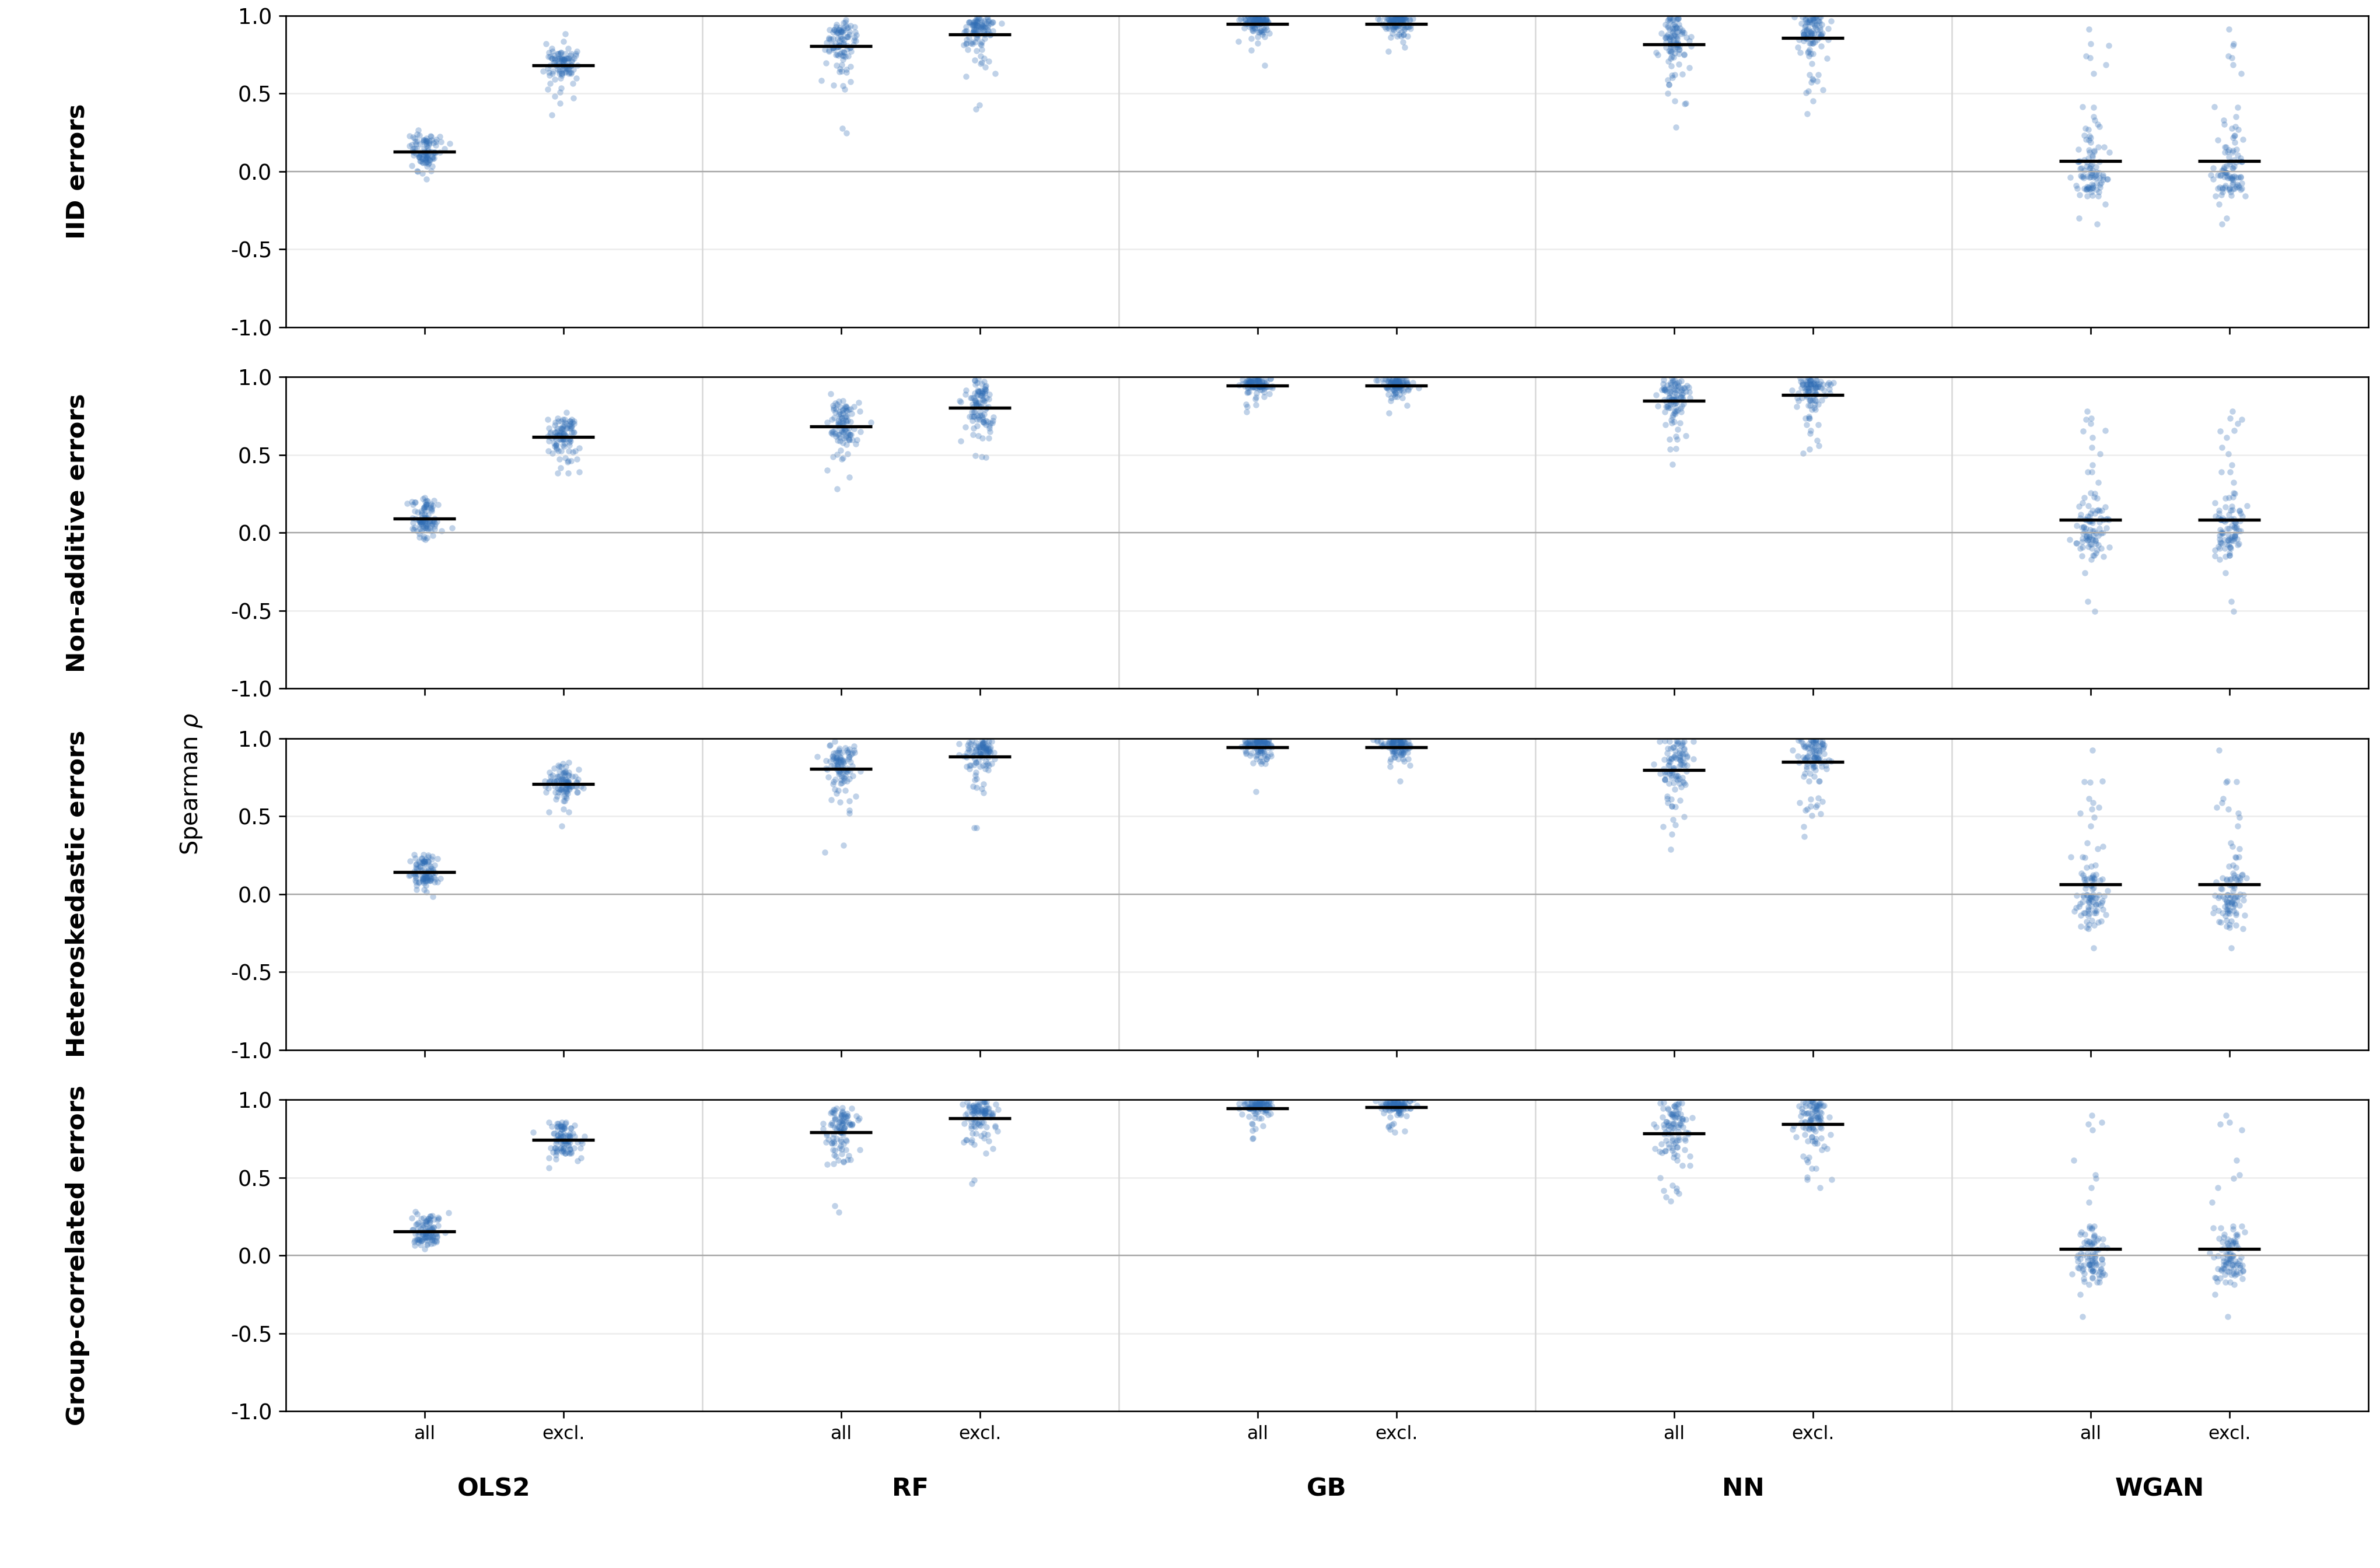
\includegraphics[width=\textwidth,height=0.445\textheight,keepaspectratio]{figures/acic_rhos_contiguous/acic_rhos_combined.png}
\par\smallskip

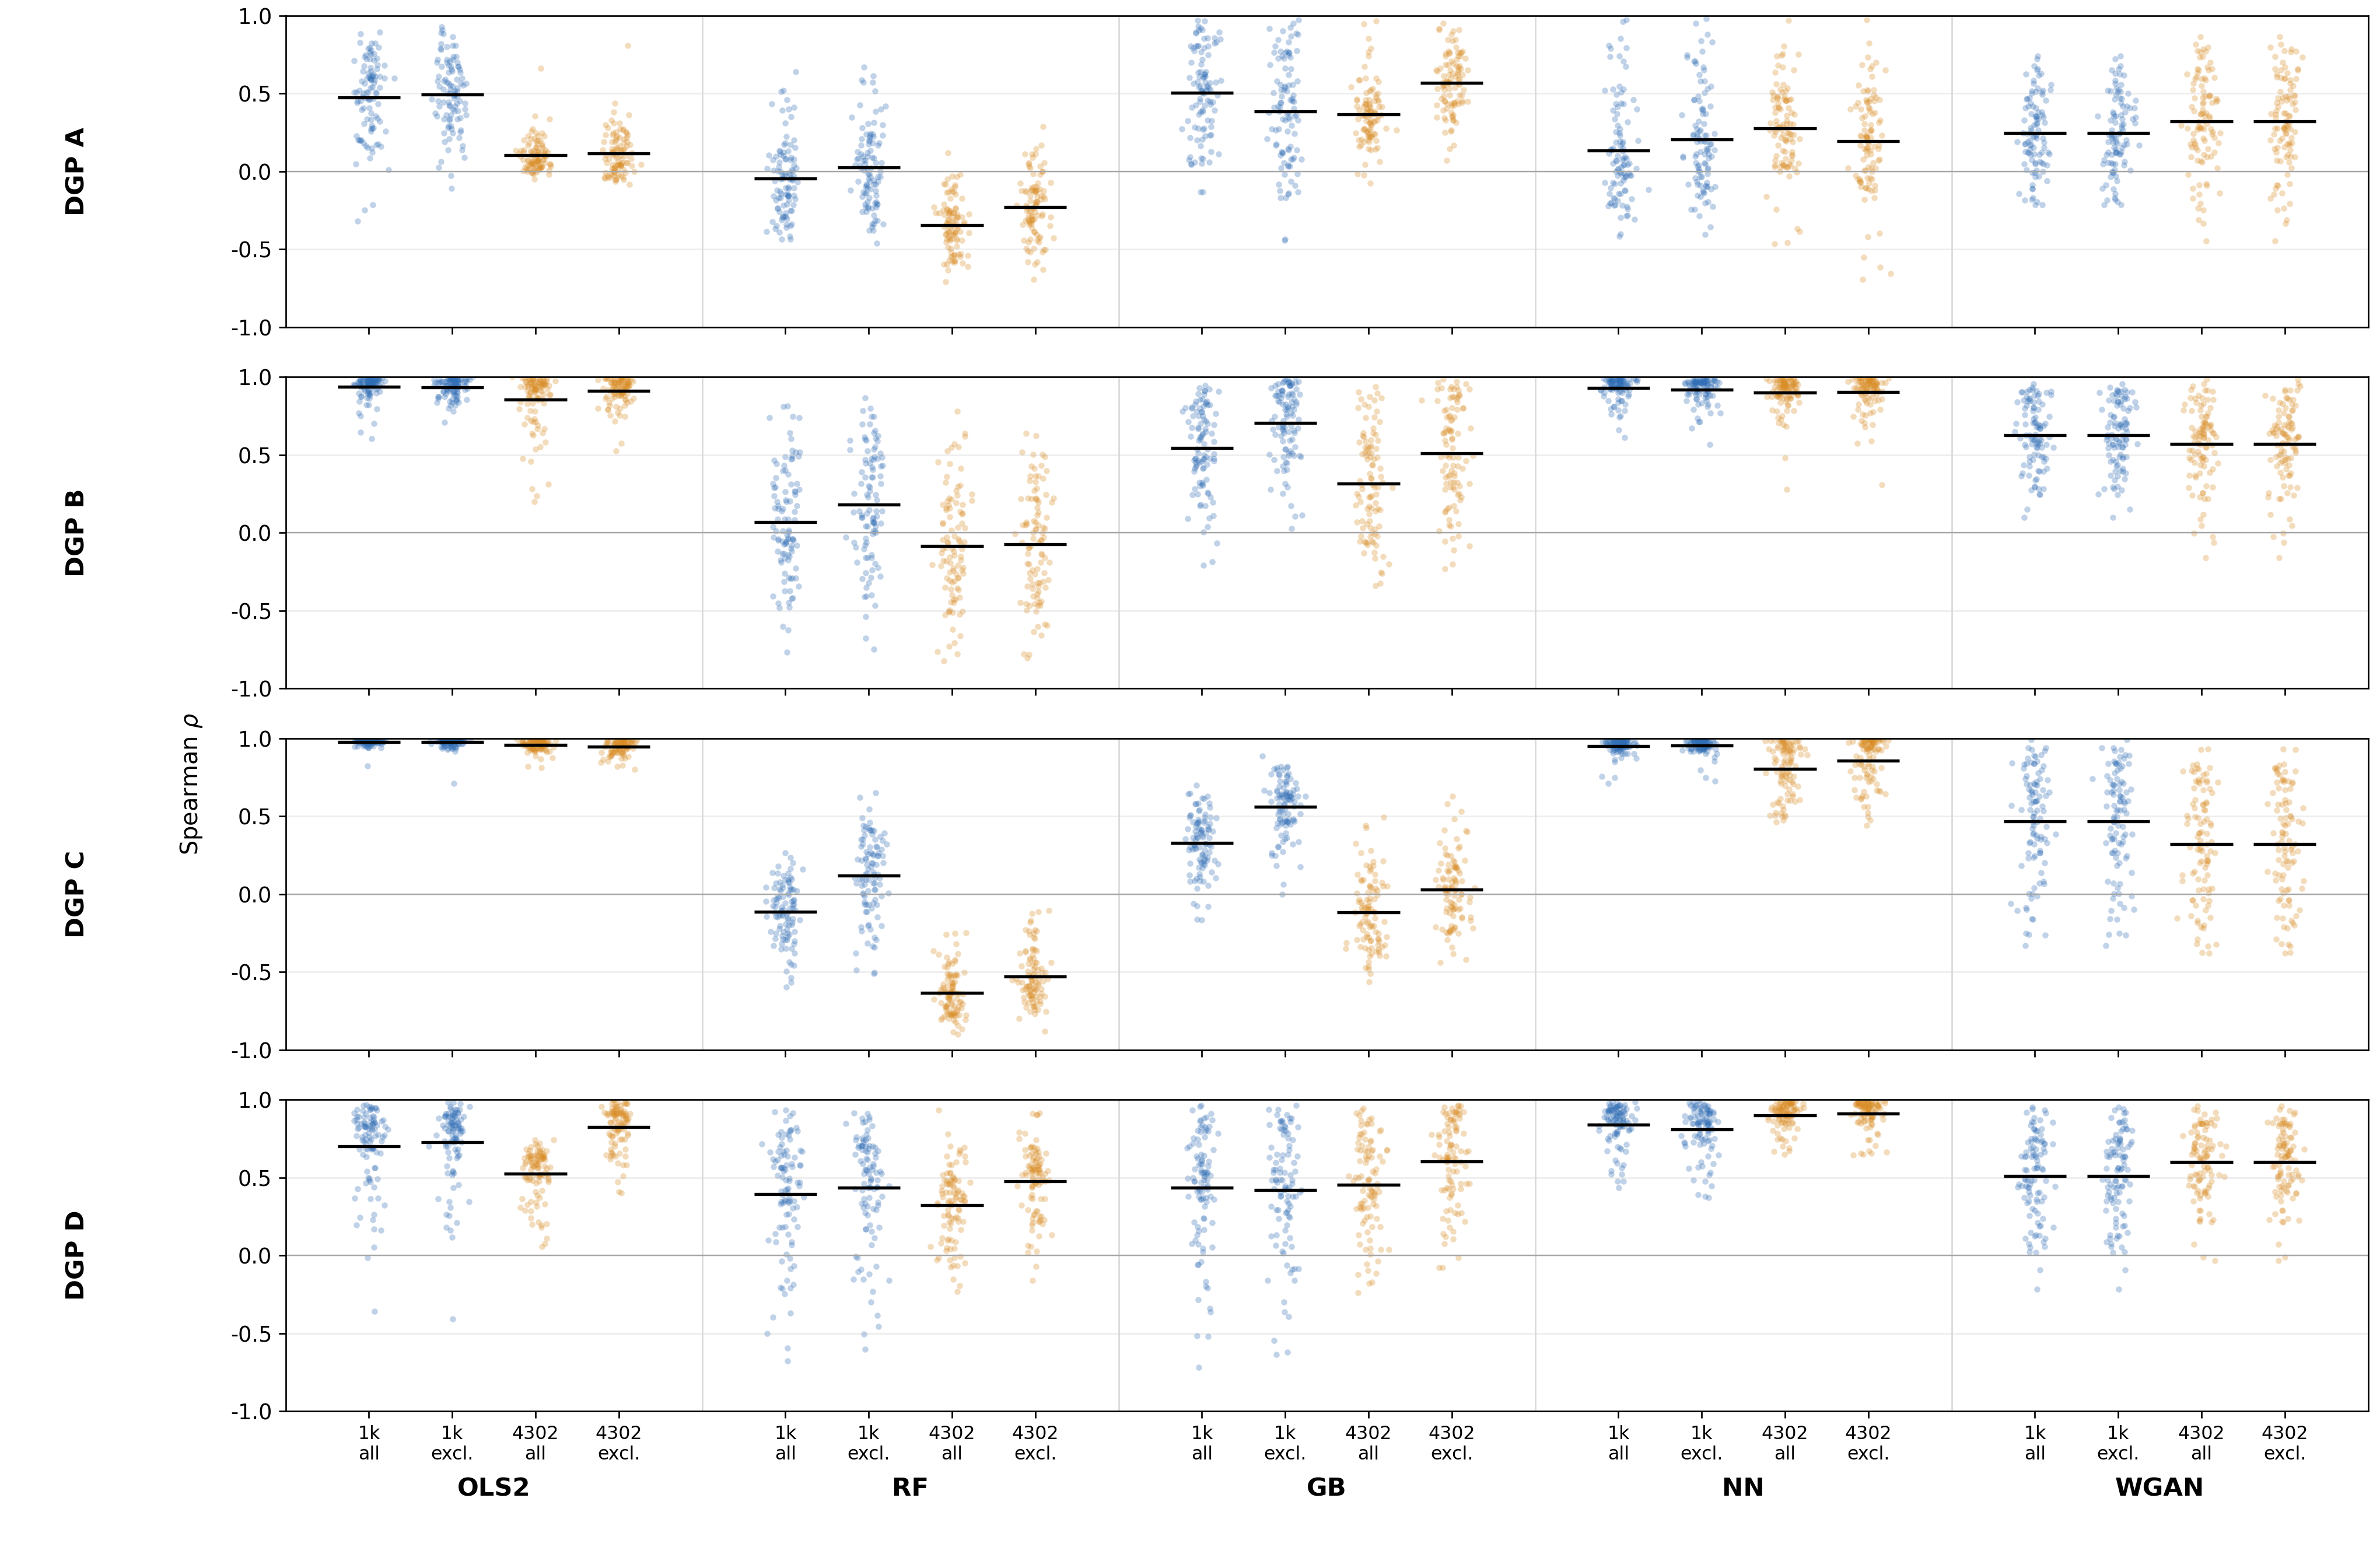
\includegraphics[width=\textwidth,height=0.445\textheight,keepaspectratio]{figures/nie_rhos_contiguous/nie_rhos_combined.png}
\caption{Per-dataset Spearman rank correlations across 100 reference datasets, using all estimators and excluding estimators sharing the simulator's outcome-model family. The upper panels show the four ACIC error structures; the lower panels show N\&W DGPs A--D, with blue and orange points denoting \(n=1000\) and \(n=4302\), respectively. Horizontal black segments indicate means.}
\label{fig:acic_rho}\label{fig:niea_rho}
\end{figure}
\FloatBarrier
\clearpage
\twocolumn
\section{Generators}
\label{app:generators}

This section describes the implementations of the original designs used to generate reference datasets before any simulator is fitted.

\subsection{ACIC 2017 designs}

The ACIC designs use the fixed \(n=4302\) covariate matrix from the Infant Health and Development Program data, with synthetic treatment and outcome mechanisms \cite{hahnAtlanticCausalInference2019}. We use the high-effect, high-noise, strong-confounding setting: \(\xi=2\), \(\eta=5/4\), and \((\kappa_1,\kappa_2)=(3,-1)\), corresponding to case 8 in their Table 2. The fitted models use eight covariates in ACIC and six in N\&W. \authorcite{hahnAtlanticCausalInference2019} distinguish the original covariate matrix from the transformed matrix used by the DGP (their Section 6.2). The formulas below use the design inputs, including indicator recodings of the cigarette-use and race variables, while retaining the original IHDP/ACIC numbering: \(X_1\) is mother's age, \(X_3\) cigarettes per day, \(X_{10}\), \(X_{14}\), and \(X_{15}\) are maternal binary health indicators, \(X_{21}\) is mother's place of birth, \(X_{24}\) is race, and \(X_{43}\) is the child's bilirubin level. Let
\[
\begin{aligned}
f(X)&=X_1+X_{43}+0.3(X_{10}-1),\\
e(X)&=\left[1+\exp\!\left\{\kappa_1f(X)+\kappa_2\right\}\right]^{-1},\\
\mu(X)&=-\sin\!\left\{F_{\!\mathcal N}^{-1}(e(X))\right\}+X_{43},\\
\tau(X)&=\xi\left\{X_3X_{24}+(X_{14}-1)-(X_{15}-1)\right\},\\
\sigma(X)&=0.4+\frac{X_{21}-1}{15},\\
\sigma_Y&=\eta\sqrt{\operatorname{Var}_n\!\left\{\mu(X)+e(X)\tau(X)\right\}},
\end{aligned}
\]
where \(F_{\!\mathcal N}^{-1}\) is the standard-normal quantile function and \(\operatorname{Var}_n\) is the variance over the fixed covariate sample. We use the quantile convention of the authors\textquotesingle{} R generator; the PDF instead prints a normal CDF in the definition of \(\mu\). For each reference dataset, treatment is redrawn independently as \(A_i\mid X_i\sim\operatorname{Bernoulli}\{e(X_i)\}\). With independent standard-normal \(\varepsilon_i\), the additive error schemes are
\[
\begin{aligned}
Y_i^{\mathrm{iid}}&=\mu(X_i)+A_i\tau(X_i)+\sigma_Y\varepsilon_i,\\
Y_i^{\mathrm{group}}&=\mu(X_i)+A_i\tau(X_i)+\sigma_Y\{0.9\varepsilon_i+0.1u_{X_{i,21}}\},\\
Y_i^{\mathrm{het}}&=\mu(X_i)+A_i\tau(X_i)+\sigma(X_i)\sigma_Y\varepsilon_i,
\end{aligned}
\]
where \(u_1,\ldots,u_{16}\) are independent standard-normal group shocks, independent of the unit-specific errors. For the non-additive design, first define
\[
\begin{aligned}
\widetilde Y_i&=\mu(X_i)+A_i\tau(X_i)+\sigma_Y\varepsilon_i,\\
a&=\frac1n\sum_{i=1}^n\{\mu(X_i)+e(X_i)\tau(X_i)\},\\
b&=1.25\sqrt{\sigma_Y^2+\operatorname{Var}_n\!\left\{\mu(X)+e(X)\tau(X)\right\}}.
\end{aligned}
\]
The observed outcome is the nonlinear transformation
\[
Y_i=13F_{\mathcal N(a,b^2)}(\widetilde Y_i)-6+\delta_i,
\qquad
\delta_i\sim\mathcal N(0,0.01^2),
\]
where \(F_{\mathcal N(a,b^2)}\) is the CDF of that normal distribution. The resulting conditional treatment effect is
\[
\begin{aligned}
\tau_{\mathrm{nonlin}}(x)
=13\Bigg[&
F_{\!\mathcal N}\!\left(
\frac{\mu(x)+\tau(x)-a}{\sqrt{\sigma_Y^2+b^2}}
\right)\\
&-F_{\!\mathcal N}\!\left(
\frac{\mu(x)-a}{\sqrt{\sigma_Y^2+b^2}}
\right)
\Bigg].
\end{aligned}
\]
\authorcite{hahnAtlanticCausalInference2019} report that the treatment-effect values accompanying the released heteroskedastic data were incorrectly calculated using the non-additive formula (their Section 6.1). Our heteroskedastic benchmark instead uses the additive outcome mechanism above and its conditional effect \(\tau(X)\), rather than those released treatment-effect values.

\subsection{N\&W designs}

For the N\&W designs \cite{nieQuasioracleEstimationHeterogeneous2021}, we use \(d=6\) covariates and generate a new \((X,A,Y)\) sample for each reference dataset. Write
\[
\begin{aligned}
Y&=b(X)+\{A-1/2\}\tau(X)+\varepsilon,\\
A\mid X&\sim\operatorname{Bernoulli}\{e(X)\},
\qquad \varepsilon\sim\mathcal N(0,1).
\end{aligned}
\]
Design A draws \(X_j\overset{\mathrm{iid}}{\sim}\operatorname{Uniform}(0,1)\); designs B--D draw \(X_j\overset{\mathrm{iid}}{\sim}\mathcal N(0,1)\). Covariates beyond \(X_5\) are noise covariates. Here \(\operatorname{trim}_{c}(u)=\min(1-c,\max(c,u))\). The functions are

\noindent\textbf{Design A}
\[
\begin{aligned}
e(X)&=\operatorname{trim}_{0.1}\!\left\{\sin(\pi X_1X_2)\right\},\\
\tau(X)&=(X_1+X_2)/2,\\
b(X)&=\sin(\pi X_1X_2)+2(X_3-0.5)^2\\
&\quad+X_4+0.5X_5.
\end{aligned}
\]
\noindent\textbf{Design B}
\[
\begin{aligned}
e(X)&=0.5,\\
\tau(X)&=X_1+\log(1+e^{X_2}),\\
b(X)&=\max\!\left\{\max(X_1+X_2,X_3),0\right\}\\
&\quad+\max(X_4+X_5,0).
\end{aligned}
\]
\noindent\textbf{Design C}
\[
\begin{aligned}
e(X)&=\{1+e^{X_2+X_3}\}^{-1},\\
\tau(X)&=1,\\
b(X)&=2\log\!\left(1+e^{X_1+X_2+X_3}\right).
\end{aligned}
\]
\noindent\textbf{Design D}
\[
\begin{aligned}
e(X)&=\{1+e^{-X_1}+e^{-X_2}\}^{-1},\\
b(X)&=\tfrac12\left[\max(X_1+X_2+X_3,0)+\max(X_4+X_5,0)\right],\\
\tau(X)&=\max(X_1+X_2+X_3,0)-\max(X_4+X_5,0).
\end{aligned}
\]

\clearpage
\section{Simulators}
\label{app:simulators}

This appendix describes the outcome models used to generate synthetic datasets within the empirical Monte Carlo design.
For generic model descriptions, we suppress the generator, reference-dataset, and Monte Carlo draw indices unless needed.

\subsection{Conditional mean--variance simulators}

Let \(\mathcal L=\{\mathrm{OLS2},\mathrm{GB},\mathrm{RF},\mathrm{NN}\}\), indexed by \(l\), be the conditional-mean outcome learners used both to construct simulators and to form causal estimators. Their conditional-mean specifications are reused for the corresponding causal estimators in Appendix~\ref{app:estimators}; the conditional-variance models below are used only to generate simulated outcomes.

The OLS2, gradient-boosting, random-forest, and neural-network simulators use a common location--scale representation that allows for heteroskedasticity,
\[
\widetilde Y_i
=
\widehat{\mu}_s(X_i,A_i)
+
\widehat{\sigma}_s(X_i,A_i)\varepsilon_i,
\]
where \(\varepsilon_i\overset{\mathrm{iid}}{\sim}\mathcal N(0,1)\). For each simulator, we obtain counterfactual conditional means
\[
\widehat{\mu}_{s,0}(X_i)
=
\widehat{\mu}_s(X_i,0),
\qquad
\widehat{\mu}_{s,1}(X_i)
=
\widehat{\mu}_s(X_i,1),
\]
and conditional standard deviations \(\widehat{\sigma}_{s,0}(X_i)\) and \(\widehat{\sigma}_{s,1}(X_i)\). A synthetic observed outcome is generated as
\[
\begin{aligned}
\widetilde Y_{i,s}^{g,m,k}
={}&
A_i^{g,m}
\left\{
\widehat{\mu}_{s,1}^{\,g,m}(X_i^{g,m})
+
\widehat{\sigma}_{s,1}^{\,g,m}(X_i^{g,m})\varepsilon_{i1}^{(k)}
\right\}\\
&+
\left(1-A_i^{g,m}\right)
\left\{
\widehat{\mu}_{s,0}^{\,g,m}(X_i^{g,m})
+
\widehat{\sigma}_{s,0}^{\,g,m}(X_i^{g,m})\varepsilon_{i0}^{(k)}
\right\}.
\end{aligned}
\]

\subsubsection{OLS2 simulator}

The OLS2 simulator fits the conditional mean as a second-order polynomial in covariates and treatment, including linear terms, squares, and all pairwise interactions. This expansion produces 54 predictor columns in ACIC and 35 in N\&W; accounting for perfect collinearities leaves 48 and 34 independent predictors, respectively, plus an intercept. The conditional variance is estimated by regressing \(\log\{(r_i^{\mathrm{OOF}})^2+\epsilon\}\) on the same terms, where \(r_i^{\mathrm{OOF}}=Y_i-\widehat\mu_{-k(i)}(X_i,A_i)\) are five-fold out-of-fold residuals and \(\epsilon=10^{-6}\widehat{\operatorname{Var}}(r^{\mathrm{OOF}})+10^{-12}\). Exponentiated predictions are rescaled so their average equals the mean squared out-of-fold residual.

\subsubsection{Gradient-boosting simulator}

The GB simulator uses \texttt{HistGradientBoostingRegressor} from Python's scikit-learn library to estimate the conditional mean of \(Y\) given \((X,A)\). Starting from \(f_0(x,a)=\overline Y\), squared-error boosting fits each regression tree \(h_b\) to the current residuals and updates the prediction:
\[
\begin{aligned}
r_{ib} &= Y_i-f_{b-1}(X_i,A_i),\\
f_b(x,a) &= f_{b-1}(x,a)+\eta h_b(x,a).
\end{aligned}
\]
Here \(\eta\) is the learning rate, and after \(B\) trees the fitted mean is \(\widehat\mu_{\mathrm{GB}}=f_B\). Both GB models use \(\eta=0.05\), at most 500 trees, and a maximum tree depth of 6, without hyperparameter tuning. Tree splits capture nonlinear effects and interactions, including interactions with treatment. Histogram binning speeds up the search for splits.

For the variance, let \(r_i^{\mathrm{OOF}}=Y_i-\widehat\mu_{-k(i)}(X_i,A_i)\) denote five-fold out-of-fold residuals, where \(-k(i)\) excludes the fold containing unit \(i\). A second GB model \(\widehat g\) predicts the log-squared residual target:
\[
\begin{aligned}
v_i &= \log\!\left[(r_i^{\mathrm{OOF}})^2+\epsilon\right],\\
\widehat\sigma_{\mathrm{GB}}^2(x,a) &= c\exp\!\left\{\widehat g(x,a)\right\}.
\end{aligned}
\]
We set \(\epsilon=10^{-6}\widehat{\operatorname{Var}}(r^{\mathrm{OOF}})+10^{-12}\), using the empirical residual variance with divisor \(n\), to keep the logarithm finite. The multiplier \(c\) makes the average predicted variance equal to the average squared out-of-fold residual.

\subsubsection{Random-forest simulator}

The RF simulator uses \texttt{RandomForestRegressor} from Python's scikit-learn library to estimate the conditional mean of \(Y\) given \((X,A)\). Each regression tree \(h_t\) is fitted to a bootstrap sample, choosing splits to reduce squared error. The forest averages the predictions of \(T\) trees:
\[
\widehat\mu_{\mathrm{RF}}(x,a)
=\frac{1}{T}\sum_{t=1}^{T}h_t(x,a).
\]
Here \(h_t(x,a)\) is the mean outcome in the leaf containing \((x,a)\). Both RF models use \(T=800\) trees, all predictors at each split, a minimum leaf size of one, and no maximum depth, without hyperparameter tuning. Tree splits capture nonlinear effects and interactions, while averaging reduces the variability of individual trees.

For the variance, let \(r_i^{\mathrm{OOB}}=Y_i-\widehat\mu_{\mathrm{OOB}}(X_i,A_i)\) denote out-of-bag residuals, where \(\widehat\mu_{\mathrm{OOB}}\) averages only trees whose bootstrap samples exclude unit \(i\). A second RF model \(\widehat g\) predicts the log-squared residual target:
\[
\begin{aligned}
v_i &= \log\!\left[(r_i^{\mathrm{OOB}})^2+\epsilon\right],\\
\widehat\sigma_{\mathrm{RF}}^2(x,a) &= c\exp\!\left\{\widehat g(x,a)\right\}.
\end{aligned}
\]
We set \(\epsilon=10^{-6}\widehat{\operatorname{Var}}(r^{\mathrm{OOB}})+10^{-12}\), using the empirical residual variance with divisor \(n\), to keep the logarithm finite. The multiplier \(c\) makes the average predicted variance equal to the average squared out-of-bag residual.

\subsubsection{Neural-network simulator}

The NN simulator uses \texttt{MLPRegressor} from Python's scikit-learn library to estimate the conditional mean of \(Y\) given \((X,A)\). After standardizing the predictors with \texttt{StandardScaler}, the network applies two hidden layers and a linear output:
\[
\begin{aligned}
h_\ell &= \operatorname{ReLU}(W_\ell h_{\ell-1}+b_\ell),\qquad \ell=1,2,\\
\widehat\mu_{\mathrm{NN}}(x,a) &= w_3^{\mathsf T}h_2+b_3.
\end{aligned}
\]
Here \(h_0\) is the standardized vector \((x,a)\), \(\operatorname{ReLU}(u)=\max(0,u)\) acts elementwise, and the weights and biases are fitted by minimizing squared-error loss with an L2 penalty. Both NN models use hidden layers of 64 and 32 units, Adam with initial learning rate \(10^{-3}\), penalty parameter \(\alpha=10^{-4}\), batch size 256, and at most 400 epochs, without hyperparameter tuning. Early stopping uses a 10\% validation split, patience of 25 epochs, and tolerance \(10^{-3}\) in validation \(R^2\). The nonlinear layers capture covariate effects and interactions.

For the variance, let \(r_i^{\mathrm{OOF}}=Y_i-\widehat\mu_{-k(i)}(X_i,A_i)\) denote five-fold out-of-fold residuals, where \(-k(i)\) excludes the fold containing unit \(i\). A second NN model \(\widehat g\) predicts the log-squared residual target:
\[
\begin{aligned}
v_i &= \log\!\left[(r_i^{\mathrm{OOF}})^2+\epsilon\right],\\
\widehat\sigma_{\mathrm{NN}}^2(x,a) &= c\exp\!\left\{\widehat g(x,a)\right\}.
\end{aligned}
\]
We set \(\epsilon=10^{-6}\widehat{\operatorname{Var}}(r^{\mathrm{OOF}})+10^{-12}\), using the empirical residual variance with divisor \(n\), to keep the logarithm finite. The multiplier \(c\) makes the average predicted variance equal to the average squared out-of-fold residual.

\subsection{Conditional generative simulator}

\noindent\textbf{Conditional Wasserstein generative adversarial network.}

We use the WGAN with gradient penalty developed by \authorcite{gulrajaniImprovedTrainingWasserstein2017}, following \authorcite{atheyUsingWassersteinGenerative2024} in fitting separate conditional models for the two treatment arms. Separate generators and critics are fitted in the control and treated groups. For treatment arm \(a\), the generator represents the conditional outcome distribution as
\[
\widetilde Y
=
G_{\theta,a}(Z,X),
\qquad
Z\sim\mathcal N(0,I).
\]
Each generator takes standardized covariates and a 10-dimensional standard-normal noise vector as inputs and has three hidden layers of 128 units with layer normalization and leaky-ReLU activations. The critic has three hidden layers of 128 units with leaky-ReLU activations and maps an outcome--covariate pair to a scalar score.

For each minibatch, the critic is updated five times to assign higher scores to observed outcomes than to generated outcomes, while the generator is updated to increase its generated outcomes' critic scores. We enforce the critic's Lipschitz constraint with the WGAN gradient penalty. Writing \(Y^G=G_{\theta,a}(Z,X)\), the losses are
\[
\begin{aligned}
\mathcal L_D
&=
\mathbb E\!\left[D_{\omega,a}(Y^G,X)\right]
-\mathbb E\!\left[D_{\omega,a}(Y,X)\right]\\
&\quad+\lambda\,
\mathbb E\!\left[\left(\left\lVert\nabla_{\bar Y}D_{\omega,a}(\bar Y,X)\right\rVert_2-1\right)^2\right],\\
\mathcal L_G
&=-\mathbb E\!\left[D_{\omega,a}(Y^G,X)\right],
\end{aligned}
\]
where \(\bar Y\) interpolates between observed and generated outcomes and \(\lambda=10\). We train each arm for 5000 epochs with batch size 512, using Adam with \((\beta_1,\beta_2)=(0,0.9)\) and learning rates \(5\times10^{-5}\) for the generator and \(2\times10^{-4}\) for the critic.

Adversarial losses do not provide a conventional convergence criterion. We therefore retain the checkpoint with the smallest average exact one-dimensional Wasserstein-1 distance between observed and generated standardized outcomes, averaged over five draws for each treatment arm. The distance is computed at the first epoch, every 200 epochs, and the final epoch.

After training, synthetic outcomes are generated by drawing new values of \(Z\) while keeping \(X_i^{g,m}\) and \(A_i^{g,m}\) fixed,
\[
\widetilde Y_{i,s}^{g,m,k}
=
G_{\widehat{\theta},A_i^{g,m}}
\left(
Z_i^{(k)},X_i^{g,m}
\right).
\]
Although the WGAN learns the full conditional distribution, its counterfactual means are needed to compute the estimand. We approximate them with \(B=10{,}000\) Monte Carlo draws per treatment and reference covariate vector,
\[
\widehat{\mu}_{s,a}^{\,g,m}(X_i^{g,m})
\approx
\frac{1}{B}
\sum_{b=1}^{B}
G_{\widehat{\theta},a}
\left(
Z_i^{(b)},X_i^{g,m}
\right).
\]

\clearpage
\section{Estimators}
\label{app:estimators}

This appendix complements the simulator description by detailing the causal estimators used in the benchmark comparison. Here \((X_i,A_i,Y_i)\) denotes unit \(i\) in the dataset to which the estimator is applied; generator, reference-dataset, simulator, and draw indices are suppressed. The outcome models that are used by some of the estimators intentionally follow the same conditional-mean specifications as the learners used to construct the simulators, \(\mathcal L=\{\mathrm{OLS2},\mathrm{GB},\mathrm{RF},\mathrm{NN}\}\). See Appendix~\ref{app:simulators} for more details.

\subsection{G-computation estimators}

For each outcome learner \(l\) in \(\mathcal L\), we estimate
\[
\widehat{\mu}_{l,a}(x)
\approx
\mathbb E[Y\mid A=a,X=x].
\]
Throughout the formulas below, \(\widehat\mu_{l,a}(X_i)\) denotes an out-of-fold prediction from a model fitted without the fold containing unit \(i\); fold indices are suppressed.
The G-computation estimator is
\[
\widehat{\Phi}_{l,\mathrm{Gcomp}}
=
\frac{1}{n}
\sum_{i=1}^{n}
\left\{
\widehat{\mu}_{l,1}(X_i)
-
\widehat{\mu}_{l,0}(X_i)
\right\}.
\]

OLS1 is a pooled additive linear regression of the outcome on treatment and covariates; its reported estimate is the treatment coefficient.

\subsection{Inverse probability weighting}
\label{app:ipw}

We estimate the propensity score, \mbox{\(e(x)=\Pr(A=1\mid X=x)\)}, using a five-fold cross-fitted \texttt{GradientBoostingClassifier} from scikit-learn, following \authorcite{chernozhukovDoubleDebiasedMachine2018}. We denote the fitted score by \(\widehat e(x)\). The classifier sequentially combines shallow trees to predict treatment status by minimizing logistic loss. We use the normalized IPW estimator \cite{luncefordStratificationWeightingPropensity2004},
\[
\widehat{\Phi}_{\mathrm{IPW}}
=
\frac{
\sum_{i=1}^{n}
A_iY_i/\widehat e(X_i)
}{
\sum_{i=1}^{n}
A_i/\widehat e(X_i)
}
-
\frac{
\sum_{i=1}^{n}
(1-A_i)Y_i/\{1-\widehat e(X_i)\}
}{
\sum_{i=1}^{n}
(1-A_i)/\{1-\widehat e(X_i)\}
}.
\]
Estimated propensity scores are truncated to \([0.01,0.99]\), corresponding to a trimming threshold of \(\delta=0.01\).

\subsection{Augmented inverse probability weighting}

For each of the outcome learners \(l\) in \(\mathcal L\), and using the same estimated propensity scores as for the IPW estimator, the AIPW estimator \cite{bangDoublyRobustEstimation2005} is
\[
\begin{aligned}
\widehat{\Phi}_{l,\mathrm{AIPW}}
={}&
\frac{1}{n}
\sum_{i=1}^{n}
\left[
\widehat{\mu}_{l,1}(X_i)
-
\widehat{\mu}_{l,0}(X_i)
\right.\\
&\left.
+
\frac{
A_i\{Y_i-\widehat{\mu}_{l,1}(X_i)\}
}{
\widehat e(X_i)
}
-
\frac{
(1-A_i)\{Y_i-\widehat{\mu}_{l,0}(X_i)\}
}{
1-\widehat e(X_i)
}
\right].
\end{aligned}
\]

\subsection{Targeted maximum likelihood estimation}

TMLE \cite{vanderlaanTargetedMaximumLikelihood2006} starts from initial estimates \(\widehat{\mu}_{l,0}(X_i)\) and \(\widehat{\mu}_{l,1}(X_i)\), for each \(l\) in \(\mathcal L\), and updates them using the estimated propensity score from the IPW estimator. For the continuous outcome considered here, define the clever covariate
\[
H_{\widehat e}(A_i,X_i)
=
\frac{A_i}{\widehat e(X_i)}
-
\frac{1-A_i}{1-\widehat e(X_i)}.
\]

The fluctuation parameter is estimated as
\[
\widehat{\varepsilon}
=
\frac{
\sum_{i=1}^{n}
H_{\widehat e}(A_i,X_i)
\left\{
Y_i-\widehat{\mu}_{l,A_i}(X_i)
\right\}
}{
\sum_{i=1}^{n}
H_{\widehat e}(A_i,X_i)^2
}.
\]
The targeted predictions are
\[
\begin{aligned}
\widehat{\mu}^{\star}_{l,1}(X_i)
&=\widehat{\mu}_{l,1}(X_i)+\frac{\widehat{\varepsilon}}{\widehat e(X_i)},\\
\widehat{\mu}^{\star}_{l,0}(X_i)
&=\widehat{\mu}_{l,0}(X_i)-\frac{\widehat{\varepsilon}}{1-\widehat e(X_i)}.
\end{aligned}
\]
The TMLE estimator is then
\[
\widehat{\Phi}_{l,\mathrm{TMLE}}
=
\frac{1}{n}
\sum_{i=1}^{n}
\left\{
\widehat{\mu}^{\star}_{l,1}(X_i)
-
\widehat{\mu}^{\star}_{l,0}(X_i)
\right\}.
\]

\subsection{Bayesian causal forest}

Bayesian causal forest (BCF) \cite{hahnBayesianRegressionTree2020} separates the outcome surface into a baseline component and a treatment-effect component:
\[
\mathbb E[Y\mid X=x,A=a]
=
\mu\{x,\widehat e(x)\}
+
a\,\tau(x).
\]
The fitted propensity score \(\widehat e(x)\) enters the baseline component. For BCF, we fit the gradient-boosting propensity model in sample, trim its predictions to the interval \([0.01,0.99]\), and standardize the outcome before fitting.

The \texttt{stochtree} algorithm represents \(\mu\) and \(\tau\) as separate sums of trees. It first performs 10 grow-from-root iterations, which construct an initial pair of tree ensembles from the data. It then runs an MCMC backfitting procedure. Conditional on the current treatment-effect forest, the baseline forest is updated using the remaining outcome residuals; conditional on the current baseline forest, the treatment-effect forest is updated using the remaining treatment-associated residuals. Thus, the trees in the two ensembles are repeatedly modified while accounting for the other component. After 20 burn-in iterations, we retain 30 posterior draws; posterior-mean potential-outcome predictions average over those draws.

We use 250 trees for the baseline forest and 50 for the treatment-effect forest. The treatment-effect forest has a shallower-tree prior (\(\alpha=0.25,\beta=3\)) than the baseline forest (\(\alpha=0.95,\beta=2\)), which shrinks effect heterogeneity more strongly than baseline outcome variation. We use the homoskedastic version of the model.

For each covariate vector, we obtain posterior-mean predictions under both treatment values, \(\widehat m(x,1)\) and \(\widehat m(x,0)\), and form
\[
\widehat\tau(x)=\widehat m(x,1)-\widehat m(x,0).
\]
The BCF G-computation estimator averages these predicted effects over the observed covariates:
\[
\widehat{\Phi}_{\mathrm{BCF}}
=
\frac{1}{n}
\sum_{i=1}^{n}
\widehat\tau(X_i).
\]

\clearpage
\section{Outcome-distribution distances}
\label{app:distances}

For each original reference dataset, let \(Y_i^0\) denote the observed outcome for unit \(i\) and \(\widetilde Y_i^{(k)}\) the outcome for that unit in the \(k\)-th dataset generated by simulator \(s\). We calculate each metric from the full samples \(\{Y_i^0\}_{i=1}^n\) and \(\{\widetilde Y_i^{(k)}\}_{i=1}^n\), then average it over the \(K\) Monte Carlo outcome draws:
\[
d_\ell^{g,m,s}=\frac{1}{K}\sum_{k=1}^{K}D_\ell\!\left(\{Y_i^0\}_{i=1}^n,\{\widetilde Y_i^{(k)}\}_{i=1}^n\right).
\]
We report three distributional distances. Writing \(F\) and \(\widetilde F\) for the two empirical CDFs, and \(Y^0_{(j)}\) and \(\widetilde Y_{(j)}\) for their ordered values, we define the distances as
\[
\begin{aligned}
W_1&=\frac{1}{n}\sum_{j=1}^{n}\left|Y^0_{(j)}-\widetilde Y_{(j)}\right|,\\
\mathrm{KS}&=\sup_y\left|F(y)-\widetilde F(y)\right|,\\
\mathrm{Energy}&=\left\{2\int_{-\infty}^{\infty}\left[F(y)-\widetilde F(y)\right]^2\,dy\right\}^{1/2}.
\end{aligned}
\]
These distances compare the full marginal outcome distributions.

Finally, within each reference dataset \(m\) and setting \(g\), we compute the Pearson correlation across the five simulators between \(d_\ell^{g,m,s}\) and their Spearman ranking fidelity \(\rho^{g,m,s}\). We report the mean of these correlations over the 100 reference datasets in each setting. Thus, simulators are compared on the same reference dataset rather than pooled across reference datasets. The alignment-excluded columns use \(\rho_{\mathrm{excl}}^{g,m,s}\), excluding estimators aligned with each simulator.
